% ---------------------------------------------------------------------------
%  A Decoupled Empathetic Response System
%  BRAC University, Department of Computer Science and Engineering, CSE400
%
%  Compile with:   pdflatex main  ->  bibtex main  ->  pdflatex main  ->  pdflatex main
%  (or simply:     latexmk -pdf main)
% ---------------------------------------------------------------------------
\documentclass[12pt,a4paper,oneside]{report}

% --- page -------------------------------------------------------------------
\usepackage[a4paper,left=1.5in,right=1in,top=1in,bottom=1in]{geometry}
\usepackage{setspace}
\onehalfspacing

% --- text -------------------------------------------------------------------
\usepackage[T1]{fontenc}
\usepackage[utf8]{inputenc}
\usepackage{lmodern}
\usepackage{microtype}

% --- figures and tables -----------------------------------------------------
\usepackage{graphicx}
\usepackage{booktabs}
\usepackage{tabularx}
\usepackage{longtable}
\usepackage{array}
\usepackage{float}
\usepackage{caption}
\captionsetup{font=small,labelfont=bf,justification=centering}

% ragged-right X columns keep long text tables from overfull lines
\renewcommand{\tabularxcolumn}[1]{>{\raggedright\arraybackslash}p{#1}}

% --- references and links ---------------------------------------------------
\usepackage[hidelinks]{hyperref}
\usepackage{cite}

\begin{document}

% ---------------------------------------------------------------------------
%  Front matter: replace with the department's official title page, declaration,
%  approval, ethics statement, acknowledgement and abstract.
% ---------------------------------------------------------------------------
\begin{titlepage}
\centering
\vspace*{1in}
{\LARGE\bfseries A Decoupled Empathetic Response System\par}
\vspace{0.4in}
{\large Emotion detection and response generation as separate stages,\\
within the memory of a consumer graphics card\par}
\vspace{0.8in}
{\large Department of Computer Science and Engineering\\
BRAC University\par}
\vspace{0.6in}
{\large \today\par}
\end{titlepage}

\pagenumbering{roman}
\tableofcontents
\listoffigures
\listoftables
\cleardoublepage

\pagenumbering{arabic}

% ---------------------------------------------------------------------------
%  Chapters
% ---------------------------------------------------------------------------
\chapter{Introduction}
\label{ch:1}

\section{Background}
\label{sec:1.1}

People are increasingly bringing their issues to the screen. A student unable to sleep the night before a viva, someone who has just lost a pet, someone who has moved to a new city and not spoken to anybody for a fortnight: all of them are likelier to type the sentence than to say it aloud. The latest global mental health estimate from the World Health Organization (WHO) indicates that there is a large and growing disconnect between the number of people who require mental health care and the services available to meet this need \cite{who2022report}. That gap is what has made text-based support -- counselling services, student helplines and everyday chat apps -- the step between having nobody to tell and seeing a professional. A response that is factually helpful but emotionally wrong, offering a solution to someone who wanted a loss acknowledged, does not merely fail to help. Empathy in text-based support is not a nebulous idea. The EPITOME framework, derived from existing empathy scales and applied to online mental-health conversations, is as much about what not to say: a series of questions turns into an interrogation \cite{samhsa2019tip35} as it is about what to say: the responses should be divided into emotional responses, their own interpretation of what the person is saying, and their speculations on what they have not yet said \cite{sharma2020epitome}. This capacity of a machine has been investigated since the inception of neural dialogue systems and the main corpus for this research is EmpatheticDialogues, a crowdsourced dataset of 24,850 dialogues, with one describing a situation related to one of 32 emotions and another responding as a listener \cite{rashkin2019,ed_github}. Two lines of work have developed out of it. The first ones learn the emotion implicitly in the layers of the neural network, such as MoEL \cite{lin2019moel} and MIME \cite{majumder2020mime} with listeners, external commonsense knowledge or graph reasoning \cite{li2020empdg,li2022kemp,sabour2022cem,zhou2023case,yang2023escm} (CEM, CASE and ESCM). The second, newer line of work is to give a large language model the tools to steer and ask it how to do so, either by prompting \cite{qian2023llm,loh2023harnessing}, by providing tools \cite{cao2025tooled}, by conditioning on personality \cite{wu2025traits} or by reasoning about emotion step by step before answering \cite{li2024emotioncot}.

The recognition of the emotion is a research issue by itself. The literature of emotion recognition in conversation has its own and its own challenges: emotions in a conversation are not always explicit and have to be deduced from the context \cite{poria2019erc}; emotions are not always read off the words in a single message, but can be implicit \cite{koga2023implicit}; a single message can have multiple emotions \cite{belay2025}; and large language models, while capable, are not necessarily more effective than a purpose-trained classifier \cite{feng2023affect}. In parallel to this, an increasing amount of work is using the same machinery for clinical screening, ranging from depression detection on social media \cite{lan2024depression} to shared tasks on mental-health timelines \cite{tseriotou2025clpsych} and systematic review shows that, despite their fluency, large language models' empathy is repetitive and obvious \cite{sorin2024jmir} and that data scarcity and bias are unsolved problems in this field \cite{kumar2024unlocking}. One thing nearly all this work has in common is that the emotional decision is never recorded. Whether the emotion is learned in the hidden layers of a joint model or inferred silently by a large language model, nobody -- not the developer, the supervisor or the clinician -- can point to it and say which feeling the reply was written for. This thesis takes the opposite position: in a system that answers feelings, the emotional decision should be a separate and visible one.

\section{Rationale of the Study or Motivation}
\label{sec:1.2}

Our motivation is practical rather than architectural. For a system like this to be adopted by a university well-being service or a small organisation, three conditions have to hold at once. It has to run on the hardware those services already own, because none of them will buy a data-centre card for a chat window. What the person typed has to stay on the machine they typed it on, because a disclosure sent to an outside service is no longer private. And somebody has to be able to look at a reply afterwards and see which feeling it was written for, because a supervisor cannot take responsibility for a decision nobody can see.

Published work satisfies at most one of the three at a time, and the following section sets out the four gaps that follow from this. Two further difficulties come from our own preliminary work rather than from the literature, and are stated as challenges in Section 1.6: a dataset that gives one emotion to a whole conversation, and a detector trained on text it will never actually be given.

\section{Problem Statement}
\label{sec:1.3}

Text-based support is now the first place many people take a difficult feeling, and the number who need such help far exceeds the number of people trained to answer them \cite{who2022report}. Whatever a service does afterwards, it must do one thing first: make the person feel understood. That is a specific job, not a vague one. A support reply has to show that the feeling has been registered, speak to the situation the person actually described, and leave room for them to say more without burying them in questions \cite{samhsa2019tip35,sharma2020epitome}. A reply that is sensible but emotionally wrong, offering a fix to someone who wanted a loss acknowledged, fails at that job however well formed its words are.

Two families of systems attempt this job, and both hide the part that matters. The joint models trained on EmpatheticDialogues learn the emotion inside their own hidden layers as a side task of generation \cite{lin2019moel,majumder2020mime,sabour2022cem,zhou2023case}; four years of architectural work moved their emotion accuracy only from 30.6\% to 41.2\%, so they still read the speaker's feeling wrongly in about three conversations out of five. The newer approach gives the whole job to a large language model and asks it to work the feeling out silently \cite{qian2023llm,loh2023harnessing}. Its replies are better and people prefer them, but its emotional judgement is no more reliable than a small purpose-trained classifier's \cite{feng2023affect,belay2025}, and it is never written down. In both families the emotional decision exists only as a passing state inside a network.

Four problems follow from this, and they compound.

\textbf{Nothing can be inspected and nothing can intervene:} because no emotion is recorded, neither a developer, a supervisor nor a clinician can ask which feeling a reply was written for, and no safeguard can sit between reading the message and writing the answer, which is the one point at which a system could decline to improvise.

\textbf{Quality is tied to scale, and scale is tied to hardware:} the strongest published results come from models too large for the equipment a university well-being service or a small charity already owns, so using them means sending what a distressed person typed to another organisation's computer. The settings that most need private, local operation are the ones that cannot have it.

\textbf{The measures reward the wrong thing:} published work is judged mainly on how far a reply overlaps in wording with one reference answer, which rewards resemblance to the corpus rather than doing what a support reply must do. It is also blind to the failure a systematic review names as the characteristic weakness of machine empathy: fluent, kind replies drawn repeatedly from the same few phrases \cite{sorin2024jmir}. A repetitive reply can sit very close to a good reference.

\textbf{Comparisons do not separate the design from the generator:} where a separated design does beat a single model, the generator has usually been changed at the same time, so the gain cannot be credited to the separation. The one published framework with a comparable two-stage structure builds it as an internal reasoning step rather than a record, and does not test it under a memory limit \cite{yang2024hef}.

The problem this thesis addresses is the combination: \textbf{the emotional reasoning of current empathetic response systems is invisible, their quality depends on hardware that most support services do not have, and the measures used to judge them do not test whether a reply does what a supportive reply is supposed to do.}

The question it asks is therefore narrow enough to answer: \textbf{does detecting the emotion in a separate, visible step produce better empathetic replies than asking one model to do both, when the whole system must fit on a single consumer GPU?} Building a working system does not answer it. Four things are needed, and this thesis is organised around them: measuring replies against what a support reply must do rather than against a reference string; holding the generator fixed so that any benefit belongs to the design rather than to model size; testing every reported difference conversation by conversation, with correction for multiple comparisons, instead of stopping at the higher average; and putting the automatic verdicts in front of people to see whether they agree.

\section{Objective}
\label{sec:1.4}

The aim of this research is to design, build and evaluate an empathetic-response system in which emotion detection and response generation are separate, independently tested components that together run on consumer hardware. Six specific objectives follow from it.

\textbf{1. Train the detector on the text it will actually receive:} fine-tune an emotion detector over the 32 categories of EmpatheticDialogues on the user's own message, rather than on the situation description the dataset supplies.

\textbf{2. Establish how the detector's output should reach the generator:} build and compare the ways of passing it on, from a single label to three candidates, per-emotion guidance and attention-derived cue words, and keep whichever measurably improves the reply.

\textbf{3. Keep the whole system within 8 GB of GPU memory:} so that it fits a graphics card people already own and no user message leaves the machine it was typed on.

\textbf{4. Evaluate against single models of both its own size and a larger one:} on five independent signals, rule adherence, an independent empathy classifier, emotional fidelity, a panel of AI judges and human raters, with every difference tested by paired statistics.

\textbf{5. Separate the design from the size of the generator:} run the system's own generator alone as a baseline, so that any gain can be credited to the separation rather than to model capacity.

\textbf{6. Show that the design is usable and not only measurable:} run it as a multi-turn conversational agent that reports the emotional decision behind every reply.

\section{Methodology in Brief}
\label{sec:1.5}

The proposed system has two parts, and the work was carried out in four steps.

The detector, d1: a RoBERTa-base encoder is fine-tuned over the 32 emotions of EmpatheticDialogues on the first message of each conversation, which is the text the system receives in use. For each message it outputs the three most likely emotions with their confidences, and the words its classification token attended to most. This backbone was chosen from five trained under identical settings.

The generator, d2: Phi-4-mini-instruct in 4-bit form, which fits beside the detector in 8 GB, produces the reply in two calls. The first is short and deterministic, asking the model to pick one of the detector's three candidates. The second builds a prompt from that one emotion, the cue words, guidance written for that emotion and three universal rules, and writes the reply. It was chosen against three generators with everything else held fixed.

The alternatives: six designs were built without a detector: zero-shot prompting, a model fine-tuned with LoRA on the listener replies from the dataset, single models of 1.5, 3.8 and 7.6 billion parameters prompted to detect and respond in one shot, and a retrieval-augmented pipeline.

The evaluation: every system answers the same 300 conversations under the same decoding settings, measured on five independent signals: automatic checks of the three response rules, the WASSA 2024 shared-task empathy classifier \cite{giorgi2024wassa,yang2024hyy33}, emotional fidelity, which reads the reply back through the detector and compares it with the conversation's emotion, two blind judges from unrelated developers \cite{zheng2023judge,verga2024}, and a human rating study. Differences are tested with paired statistics and corrected for multiple comparisons. Chapter 4 gives the full design.

\section{Scopes and Challenges}
\label{sec:1.6}

 \textbf{Scopes:}

\textbf{1. Emotionally aware support on ordinary hardware: }the complete system runs inside 8 GB of GPU memory, so a user's disclosure never has to leave the machine it was typed on.

\textbf{2. An inspectable emotional decision:} each answer carries an audit trail, the three emotions with their confidences, the one selected, and the words behind the detection, which a single end-to-end model cannot produce.

\textbf{3. Replaceable components: }the detector, the per-emotion guidance and the generator can each be swapped without disturbing the others, as we show by substituting a larger detector into the finished system.

\textbf{4. Not only a benchmark entry, but a multi-turn agent: }the same components run as a conversational agent that reads the user's previous turns and relaxes its rules after the first.

\textbf{5. Evaluation relative to the use case:} replies are judged on the rules, an independent empathy classifier, a judge panel and human raters, not on similarity to a reference reply.

\textbf{6. Reproducibility: }every parameter, seed and measurement is recorded, and all tables and figures are generated by script from the saved outputs.

\textbf{ Challenges:}

\textbf{1. One label for a collection of emotions: }the dataset gives a whole conversation one emotion, though a message may carry several, so a detector trained on it can only ever be asked for one.

\textbf{2. Training text against deployment text: }the detector was first trained on text unlike the text it receives in use, costing about nine points of accuracy until the mismatch was found and corrected.

\textbf{3. A memory budget that leaves no room to spare: }both models share 8 GB, which forces 4-bit quantisation and rules out the larger generators used in published work.

\textbf{4. Measures that reward length: }both the empathy classifier and the judges score longer replies higher, so comparisons between systems of different verbosity need care.

\textbf{5. Judges that may favour their own kind: }models used as evaluators tend to prefer text from their own family \cite{panickssery2024}, which restricts which of them may judge which systems.

\textbf{6. No category for crisis: }nothing in the emotion set matches suicidal ideation, and the system must not be used as a mental-health service.

\section{Thesis Structure}
\label{sec:1.7}

\textbf{Chapter 1} gives the background to empathetic response generation and text-based support, the motivation, the problem, the objectives, a brief account of the methodology, and the scopes and challenges of the work.

\textbf{Chapter 2} reviews the literature: the preliminaries of empathetic dialogue and emotion recognition, the model families used here, existing work with purpose-built models and with large language models, and the findings and gaps that follow.

\textbf{Chapter 3} sets out the requirements and specifications, the societal and environmental impacts, the ethical aspects, the standards followed, the project and risk management plans, and the economic analysis.

\textbf{Chapter 4} presents the methodology: the design process, every design considered, the detector and generator candidates, the ways of connecting them, the designs built without a detector, the preparation of the data, and the implementation of the selected design.

\textbf{Chapter 5} reports the results: how each system performed on the same conversations, the analysis of the design alternatives, the adjustments made to the final design, the statistics behind every reported difference, the comparison with published work, and what the results do and do not establish.

\textbf{Chapter 6} concludes, summarising the findings, stating the contributions and recommending future work.

\chapter{Literature Review}
\label{ch:2}

\section{Preliminaries}
\label{sec:2.1}

\textbf{Empathy as something that can be measured:} a system cannot be built against a vague word. This work uses EPITOME for text-based mental-health support, built on well-known empathy scales, which divides a reply into \textit{emotional reactions}, naming and validating the feeling; \textit{interpretations}, showing the situation has been understood; and \textit{explorations}, inviting the person to say more \cite{sharma2020epitome}. Counselling practice adds the opposite limit, warning of the question-and-answer trap in which the person becomes a passive respondent \cite{samhsa2019tip35}. Together they give a working definition a machine can be held to: acknowledge the feeling, respond to the situation, and invite without interrogating.

\textbf{The corpus:} EmpatheticDialogues is the standard benchmark for this task \cite{rashkin2019}. One crowdworker was given one of 32 emotion labels, wrote a description of a matching situation and then described it in conversation, while a second replied as a listener without seeing the label. The released files hold 24,850 conversations split so that no speaker appears in more than one set \cite{ed_github}. Two features matter here: the situation description and the first message are distinct texts, the description written first; and each conversation carries exactly one label, chosen before it was composed.

\textbf{GoEmotions }is the other dataset commonly used for fine-grained emotion: about 58,000 Reddit comments labelled with 27 emotions plus neutral, allowing more than one label per comment \cite{demszky2020}. This project began there and moved to EmpatheticDialogues for four reasons measured in Section 4.3.1.

\textbf{Emotion recognition in conversation} is a field of its own rather than sentence-level classification, because the same words carry different feelings depending on what preceded them \cite{poria2019erc}. Related work classifies the intents a listener's reply can express on the same corpus \cite{welivita2020}, and shows that emotions in dialogue are often implied and must be inferred rather than read off \cite{koga2023implicit}, and that one reply can carry more than one label \cite{belay2025}.

\textbf{Models:} every model here derives from the transformer \cite{vaswani2017}, in two families doing two jobs. \textbf{Encoders }are trained with masked-language modelling, which suits them to classification; BERT set the precedent \cite{devlin2019} and RoBERTa extended it with more text, longer training and dynamic masking \cite{liu2019roberta}. \textbf{Decoder-only language models} generate text left to right and, when instruction-tuned, follow written instructions; we use Qwen2.5 \cite{qwen2024} and Phi-4-mini \cite{abouelenin2025phi4mini}, the latter trained with a particular emphasis on instruction following.

\textbf{Two techniques bring large models to size} on a consumer GPU. \textbf{Quantisation }stores weights at reduced precision; 4-bit NF4 with double quantisation keeps the quality of 16-bit weights at roughly a quarter of the memory \cite{dettmers2023qlora}. \textbf{Low-rank adaptation} trains a small set of extra parameters rather than the whole network, making fine-tuning feasible on the same hardware \cite{hu2022lora}. A third, \textbf{retrieval-augmented generation}, supplies relevant passages retrieved at inference time \cite{lewis2020rag}, usually through sentence embeddings \cite{reimers2019sbert}; this work uses it as a baseline but not in the final design.

\textbf{Measure of empathy:} no single automatic measure captures empathy, so three kinds of evaluation are used here. The\textbf{ WASSA shared task on empathy detection }provides a model trained on human empathy ratings of conversation turns \cite{giorgi2024wassa}, used here as the hyy33 system \cite{yang2024hyy33}.\textbf{ Large language models as judges} track human preference well when the judge is strong \cite{zheng2023judge} but favour their own generations \cite{panickssery2024}, so a panel from different developers is recommended over a single judge \cite{verga2024}. The reference remains \textbf{human evaluation}, reported either as a five-point rating \cite{qian2023llm} or a head-to-head preference \cite{cao2025tooled}.

\section{Review of Existing Research}
\label{sec:2.2}

The relevant work falls into six groups: the benchmark that began the field; the models trained end to end on it; work on the listener rather than the speaker; the arrival of large language models, which changed what counts as a good reply; the narrower but decisive question of whether those models recognise emotion or only write about it well; and the clinical work using the same machinery for screening rather than replying. Two further sections cover the study closest to ours and how any of this should be judged.

\subsection{The Benchmark That Created the Field}
\label{sec:2.2.1}

Rashkin et al. (2019) created the field by releasing EmpatheticDialogues with a framing every later paper has followed: a listener answers a person's description of an emotional situation, and the emotion is one of 32 fine-grained categories rather than a sentiment \cite{rashkin2019}. That choice is why top-1 accuracy here sits far below figures on two- or six-class tasks: it forces a system to separate feelings a sentiment model would merge, such as \textit{sad}, \textit{lonely}, \textit{disappointed }and \textit{devastated}.

Two further decisions in that paper shaped everything after it. The emotion label may either be given to the generator or predicted by it, and the paper shows both. And it set a reference point for recognition: a fastText classifier at about 43\% accuracy \cite{rashkin2019}. That figure is widely cited, and it was measured on the situation description, the text the crowdworker wrote about the event, not on the first message the speaker sends the listener. The two differ in length and explicitness, since a description of an event names the feeling more openly than a message written to another person. Any system working on what a user actually types is solving the harder of the two problems, and Section 5.2.2 gives our own measurement of that gap.

\subsection{Joint Models Trained End to End}
\label{sec:2.2.2}

A series of \textbf{joint models} followed, each adding a mechanism to a single encoder-decoder network trained from scratch on the corpus. MoEL (Lin et al., 2019) used a mixture of listeners, one per emotion, fused by a softmax over the detected emotion so the model could answer different feelings differently \cite{lin2019moel}. MIME (Majumder et al., 2020) started from an observation about human listeners, that they partly mirror the speaker's emotion and partly compensate for it \cite{majumder2020mime}. EmpDG (Li et al., 2020) added an adversarial discriminator judging whether a reply looked empathetic, together with emotion signals at more than one granularity \cite{li2020empdg}. The next three brought in knowledge the corpus does not contain. KEMP (Li et al., 2022) added external commonsense and concept knowledge, letting the model infer about the situation rather than only its words \cite{li2022kemp}. CEM (Sabour et al., 2022) directed those inferences at the speaker, eliciting their likely reactions, intentions and needs \cite{sabour2022cem}. CASE (Zhou et al., 2023) aligned a commonsense graph with a concept graph, on the view that a listener must relate what the speaker thinks to what they feel \cite{zhou2023case}. ESCM (Yang et al., 2023) then used emotion-semantic vectors that change across the conversation, supervised explicitly on the emotional signal \cite{yang2023escm}.

Read in order, these papers show emotion accuracy creeping up: 30.6\% for EmpDG, 30.8\% for MoEL, 36.6\% for KEMP, 37.8\% for CEM, 38.9\% for CASE and 41.2\% for ESCM. Two things follow. The gains come from added knowledge and structure rather than from what is done with the emotion once predicted; and after four years of architectural work the best of them still misreads the speaker's feeling in about three cases out of five. A related model suggests why. Liu et al. (2021) ran RoBERTa-GPT2 on the same task and corpus but initialised its encoder from pre-trained RoBERTa and its decoder from pre-trained GPT-2 instead of training from scratch, reaching 51.5\% \cite{liu2021robertagpt2}, about ten points above the best knowledge-augmented model here. On a corpus this size the limiting factor was not what was built into the models but how little text they had seen, which is the first reason our design spends its parameter budget on strong pre-trained components and on how they are connected.

\subsection{The Listener's Side of the Conversation}
\label{sec:2.2.3}

Most of the above models the speaker. A smaller body of work looks at the listener instead, and for a rule-based design it is more useful than its citation count suggests. From a large sample of EmpatheticDialogues, Welivita and Pu (2020) built a taxonomy of empathetic response intents showing that the listeners in this corpus use a small, describable set of behaviours: questioning, acknowledging, consoling, agreeing, encouraging, sympathising and a few more \cite{welivita2020}. That matters for any rule-writing approach, ours included, because it shows supportive replies have structure. If human listeners work from a short list of moves, asking a generator to name the feeling, answer the situation and ask no more than one question is not an arbitrary constraint but a description of what the corpus already does.

The wider literature on emotion recognition in conversation supplies the other half. Poria et al. (2019) explain why it is not sentence-level classification: the same words carry different feelings depending on what precedes them, so context is an input to the system rather than an optional extra \cite{poria2019erc}. That is why how much conversation the detector reads is treated here as a parameter to be measured rather than assumed, as reported in Section 5.3.2.

\subsection{Large Language Models Enter the Task}
\label{sec:2.2.4}

\textbf{Large language models} changed the field, and Qian et al. (2023) made that plain. Their human evaluation of ChatGPT against the purpose-built models above found raters overwhelmingly favouring ChatGPT, 4.64 out of 5 against 3.08 for CEM \cite{qian2023llm}, a gap tuning cannot explain. The paper then took a path directly relevant to our design: replies improve when the emotion is given explicitly, and improve further when the model is told to reason about the situation before answering. The best system in this literature was therefore a general model given structure from outside, which is what our two-stage pipeline supplies. Loh and Raamkumar (2023) reached a similar conclusion against counselling criteria for online mental-health support, adding that without structure the replies stay generic \cite{loh2023harnessing}.

That structure takes several forms, each with a price. TOOL-ED (Cao et al., 2025) treats a commonsense knowledge base as a tool the model may call during generation, deciding when to consult COMET or CICERO rather than having their output injected into every input, which avoids the noise unrestricted knowledge introduces and frees the system from any one knowledge base \cite{cao2025tooled}. It is the knowledge built into KEMP and CEM, now pulled as needed. The cost shows in the setup: a fine-tuned 7B model trained on 48 GB GPUs \cite{cao2025tooled}, six times our GPU memory.

Wu et al. (2025) argue the same situation should be answered differently for different people, conditioning generation on an MBTI classifier of about 84\% accuracy and on images alongside the text \cite{wu2025traits}. Their model reaches 45.4\% emotion accuracy, dropping almost 4 points without the personality signal \cite{wu2025traits}. The constraint for our aim is the input: the design assumes visual data and personality labels, and a text-only system reading a single message has neither.

Wang et al. (2025) entered the NLPCC 2025 emotional support conversation task, where the target is a strategy sustained across a conversation, comparing low-rank adaptation with full fine-tuning on Qwen2.5 \cite{wang2025esc}. Two facts apply here. Their best configuration raised the combined score from 30.87 to 41.17 using low-rank adaptation, with the adapter's rank and scaling factor affecting the score \cite{wang2025esc}, and their settings bracket ours (Section 4.4.4). The other is scale: the entry fine-tuned models up to 72B parameters on 1,500 dialogues, the opposite end of the resource question from the system built here.

Rasool et al. (2025) work on psychotherapy transcripts rather than crowdsourced conversations, injecting emotion-aware embeddings at word, sentence and session level into Flan-T5, Llama 2 13B, DeepSeek-R1 and GPT-4, with a vector index retrieving related passages over those embeddings \cite{rasool2025}. The retrieval part resembles the baseline this thesis builds from sentence embeddings at generation time \cite{reimers2019sbert,lewis2020rag}, and is a useful comparison for Section 5.2.5, where our retrieval variant is measured and rejected. They report gains in empathy, coherence and fluency over their baselines, but note that their paired significance tests fall short of the conventional threshold and that the study has no human evaluation \cite{rasool2025}. Li et al. (2024) take the emotional route instead of the knowledge one, having the model reason step by step about emotion before answering \cite{li2024emotioncot}; our stage-one emotion choice is a condensed form of the same idea, one deliberate choice, recorded, before any reply is written.

\subsection{Do These Models Recognise Emotion?}
\label{sec:2.2.5}

All of that concerns the quality of the answers. Whether large models reliably \textit{detect }emotion is a separate question, and the one this thesis turns on, since a decoupled design is only worth building if a dedicated detector is genuinely better. The evidence says it is.

Feng et al. (2023) tested large language models on affect recognition in conversation and found them comparable to, not better than, purpose-trained classifiers \cite{feng2023affect}. Belay et al. (2025) settled the comparison, building a multi-label emotion dataset in four Ethiopian languages (EthioEmo), adding the English SemEval-2018 data, and comparing encoder-only, encoder-decoder and decoder-only models together with in-context learning. Their conclusion is plain: fine-tuned smaller pre-trained models beat the zero-shot performance of large language models on this task, the best decoder-only averaging about 46 against about 72 for a fine-tuned encoder on its best language \cite{belay2025}. They also find that correct multi-label classification remains hard even in English, and that well-resourced and poorly resourced languages differ sharply \cite{belay2025}, a point we return to in Section 5.6.5, since our system is English only.

Two further papers explain \textit{why }recognition is hard rather than \textit{how well} it is done. Koga et al. (2023) studied emotions that are evoked but not expressed and concluded that much of the problem is inference rather than classification \cite{koga2023implicit}. The second difficulty is Belay et al.'s own, that an utterance often carries more than one emotion at once \cite{belay2025}, which is one reason our detector returns three candidates instead of one.

The best single figure comes not from a benchmark paper but from a deployed system. The Chirpy Cardinal agent built for the Alexa Prize carried a RoBERTa classifier over the same 32 categories, reported at about 61.5\% accuracy on the first utterance, with errors concentrated on neighbouring emotions rather than scattered \cite{paranjape2020chirpy}. Our results reproduce both parts: Section 5.1.2 reports the accuracy and the same neighbour-heavy error pattern, which is what makes a three-candidate output useful rather than evasive, and Section 5.5.1 explains the difference between the two figures.

\subsection{Clinical and Mental-Health Applications}
\label{sec:2.2.6}

The clinical end of the field uses the same machinery for screening rather than replying, and sets the standard of care such a system will be held to. Lan et al. (2024) applied large language models to depression detection on social media \cite{lan2024depression}, and the CLPsych 2025 shared task recast the problem as tracking mental-health dynamics across a user's timeline rather than classifying a single post \cite{tseriotou2025clpsych}. Kumar et al. (2024) survey the two problems limiting the area: labelled clinical data is scarce, and the bias from training on what little exists is hard to detect \cite{kumar2024unlocking}.

The caution most relevant to our design comes from the systematic review by Sorin et al. (2024), which we act on directly. That large language models were often scored as empathetic as clinicians or more so, across the studies it examined, is remarkable in itself. The problem the review identifies is not incompetence but sameness: the empathy was repetitive, the same formulations recurring across answers \cite{sorin2024jmir}. A comparison with a reference cannot detect that failure, since a repetitive reply may sit very close to a good one. Hence the repetition measure among our own signals in Section 5.1.4, which none of the joint models above reports.

\subsection{The Closest Prior Work}
\label{sec:2.2.7}

The study most similar to this thesis is the \textbf{Hybrid Empathetic Framework} by Yang et al. (2024). It first adds a small, specialised empathetic model to a large language model, and then predicts the emotion in two steps, along with determining the reason for the emotion \cite{yang2024hef}. That's the same architectural intuition that this thesis seeks to achieve: a small model that is good at emotion feeding a large model that is good at language, with the emotional decision made in a stage of its own, not folded into generation.

The systems differ in purpose. Their framework targets benchmark performance on empathetic generation. Ours runs entirely within 8 GB on a consumer GPU so a user's disclosure never leaves the machine; exposes the whole emotional decision, the candidates, their confidence and the words behind them, as an audit trail on every reply; and judges replies by what a supportive reply must do rather than by how closely they match a reference. Because that paper exists, our contribution is not the idea of separating detection from generation, but what the separation provides and the evidence gathered for it.

Table~\ref{tab:2.1} compares the works that are most similar to this thesis side by side, what each used, what each accomplished, and the limitation that is pertinent here.

\begin{table}[htbp]
\centering
\footnotesize
\caption{Works that are most similar to this thesis and limitation of each work}
\label{tab:2.1}
\begin{tabularx}{\textwidth}{@{}lXXX@{}}
\toprule
\textbf{Work} & \textbf{Data} & \textbf{Approach and result} & \textbf{Limitation relevant to this thesis} \\
\midrule
Rashkin et al., 2019 (ACL) & EmpatheticDialogues & Introduces 25k-conversation, 32-emotion benchmark; emotion classifiers on situation text & Benchmark only; situation-text classifiers overstate real-input accuracy \\
Lin et al., 2019 - MoEL (EMNLP) & ED & Mixture of emotion-specific listeners; emotion acc 30.75\% & Low recognition accuracy; small model generation \\
Majumder et al., 2020 - MIME (EMNLP) & ED & Emotion mimicry grouped by polarity & Coarse polarity groups; generic replies \\
Sabour et al., 2022 - CEM (AAAI) & ED & Adds COMET commonsense (cognitive + affective) & Human empathy 3.08/5, far below LLMs \\
Zhou et al., 2023 - CASE (ACL) & ED & Aligns cognition and affection at coarse and fine grain & Human empathy 3.04/5 \\
Qian et al., 2023 (arXiv 2310.05140) & ED & LLMs (ChatGPT) beat trained SOTA on automatic and human metrics & Uncontrolled, verbose; no rule/format control measured \\
Paranjape et al., 2020 - Chirpy Cardinal & ED + live Alexa users & RoBERTa-large emotion classifier on first utterance, 61.5\% top-1 & Technical report; validation-set score \\
Cao et al., 2025 - TOOL-ED (COLING) & ED & LLM tool-calling for commonsense knowledge; A/B human eval & Fine-tuning 7-14B models; heavy resources \\
Wu et al., 2025 - Personality-aware ERG (COLING) & MELD-based multimodal + ED & Personality + visual cues; emotion acc 45.4\% text-only & Needs multimodal input and personality labels \\
Belay et al., 2025 (COLING) & EthioEmo (4 Ethiopian languages) + SemEval-2018 English & Encoder, encoder-decoder, decoder LLMs for multi-label emotion & Fine-tuned encoders still beat few-shot LLMs at emotion classification \\
Rasool et al., 2025 (AI, MDPI) & Psychotherapy transcripts & Emotion-aware embedding fusion into Flan-T5/Llama 2/DeepSeek-R1/GPT-4; BERT for emotion & Paired t-tests non-significant; no human evaluation \\
Wang et al., 2025 (arXiv 2507.12820) & NLPCC 2025 ESC task & Prompting + LoRA / full fine-tuning of Qwen2.5; total 41.17 vs 30.87 base, ranked 2nd & Needs fine-tuning up to 72B parameters \\
\bottomrule
\end{tabularx}
\end{table}

\subsection{How Empathetic Replies Should Be Judged}
\label{sec:2.2.8}

Finally, \textbf{how this should be measured} has become a literature of its own, and it is where this thesis departs furthest from the earlier papers, since our question can only be answered by measurement.

Zheng et al. (2023) found strong language models used as judges agreeing with human preference over 80\% of the time, comparable to agreement between people, and documented their shared biases, such as a preference for longer answers \cite{zheng2023judge}. Panickssery et al. (2024) showed that such evaluators recognise and favour their own generations, making the choice of evaluator a methodological decision rather than a convenience, since a judge from the same family as a system under test is not a neutral instrument \cite{panickssery2024}. The remedy this thesis adopts, a panel of judges from different model families, was proposed by Verga et al. (2024) on grounds of both reduced bias and lower cost \cite{verga2024}.

The complementary solution is to train a model directly on human empathy ratings rather than have it imitate a rater \cite{giorgi2024wassa}, as in the hyy33 system used here \cite{yang2024hyy33}; its value is being unrelated to every system evaluated. Human evaluation remains the benchmark, reported recently either as a five-point rating \cite{qian2023llm} or a head-to-head comparison \cite{cao2025tooled}. This thesis uses all three, with the judges and the classifier in one panel, standardised before averaging (Section 5.1.5).

\section{Summary of Key Findings}
\label{sec:2.3}

The review yields seven findings, each stated with its evidence and with what this thesis does about it.

\textbf{Pre-training matters more than architecture for this task:} four years of joint models moved emotion accuracy from 30.6\% to 41.2\% \cite{lin2019moel,majumder2020mime,li2020empdg,li2022kemp,sabour2022cem,zhou2023case,yang2023escm}, while RoBERTa-GPT2 reaches 51.5\% on the same task simply by using pre-trained components instead of training from scratch \cite{liu2021robertagpt2}. Ten points separate them and the cheaper method wins, so the parameter budget is better spent on a strong pre-trained model, and on how it is connected, than on a network built from 25,000 conversations.

\textbf{Large language models write better replies than purpose-built empathy models but do not reliably detect emotion: }human raters prefer ChatGPT to CEM, 4.64 against 3.08 \cite{qian2023llm}, and a systematic review finds large models rated level with or above clinicians on empathy \cite{sorin2024jmir}. Yet they do no better than trained classifiers on conversational affect \cite{feng2023affect}, worse than fine-tuned encoders on multi-label emotion \cite{belay2025}, and struggle with implied emotion \cite{koga2023implicit}. That asymmetry is the direct argument for a separate detector and a generator doing only what it is good at.

\textbf{A small fine-tuned model can beat a large prompted one at classification: }the sharpest evidence for our architecture comes from outside the empathy literature. Belay et al. found fine-tuned smaller models still beating the zero-shot performance of large language models on the same multi-label dataset \cite{belay2025}, and our own corpus has a matching figure, a RoBERTa classifier at about 61.5\% on the 32 EmpatheticDialogues emotions \cite{paranjape2020chirpy}. A detector of a few hundred million parameters is therefore not a hardware compromise but, on this task, the better instrument.

\textbf{Machine empathy is repetitive and hardly anyone measures it: }the weakness the systematic review identifies is not incompetence but sameness, fluent and kind replies drawn from a small pool of phrases \cite{sorin2024jmir}. None of the joint models above reports a repetition measure, and a reference-based comparison cannot find the problem, since a repeated reply may sit close to the reference. We therefore report repetition for every system, not only ours.

\textbf{Structure helps, and there are several ways to supply it, each with a cost: }telling the model the emotion or asking it to reason before answering \cite{qian2023llm,li2024emotioncot}; offering a knowledge base as a callable tool \cite{cao2025tooled}; conditioning on inferred personality and visual input \cite{wu2025traits}; fine-tuning with a low-rank adapter \cite{wang2025esc}; or retrieving related passages at generation time \cite{lewis2020rag,rasool2025}. All report gains, but none establishes what is worth its cost under a hardware constraint: tool calling needs 48 GB \cite{cao2025tooled}, the fine-tuned approach models up to 72B parameters \cite{wang2025esc}, and the trait-aware approach multimodal input with personality labels \cite{wu2025traits}. Chapter 5 answers that within 8 GB, including the retrieval variant, which we measure and dismiss.

\textbf{Evaluation is the field's weakest aspect, and workable alternatives now exist: }published comparisons rest on overlap with a single reference reply, which cannot tell whether a reply acknowledged the feeling or asked five questions in a row, and one recent study reports improvements that miss the conventional threshold and that no human rated \cite{rasool2025}. The alternatives include a classifier trained directly on human empathy ratings \cite{giorgi2024wassa,yang2024hyy33} and panels of judges from different developers, which offset the self-preference any single judge shows \cite{zheng2023judge,verga2024,panickssery2024}. They let this thesis judge replies by what they \textit{do} rather than what they resemble.

\textbf{Separating a small model from a large one has been proposed, but for another purpose: }the Hybrid Empathetic Framework pairs a small empathetic model with a large one and predicts the emotion in two steps \cite{yang2024hef}. Our work shares that structure and differs in purpose: a whole system within 8 GB, the emotion exposed as an auditable record rather than an internal step, and an evaluation built on rule adherence, an empathy panel and paired statistics.

\textbf{The gap this thesis fills:} to our knowledge no existing work builds an empathetic response system that (i) runs entirely on consumer hardware, so nothing a user discloses leaves the machine, (ii) exposes its whole emotional decision for inspection before a reply is written, and (iii) is evaluated against single-model baselines of both its own size and a larger one, on measures matching what a supportive reply must do, with every difference tested statistically. Chapters 4 and 5 build and test that system.

\chapter{Requirements, Impacts and Constraints}
\label{ch:3}

More than accuracy is judged by a system that responds to people describing painful experiences. It should function with the hardware that a student team owns, it should not use the data it learns from in a way that violates the licence of the data, it should not misuse anything a person types to it, and it should never pretend to be providing any kind of help that it is not qualified to provide. This chapter outlines the requirements that were designed to address those demands and the potential impact the system may have on people and the environment, as well as the ethical considerations imposed upon the system, what standards are adhered to, and how the project was planned and the risks and costs managed.

\section{Final Specifications and Requirements}
\label{sec:3.1}

This work needed to meet both technical and methodological requirements. Technically, two models needed to run in parallel on a single consumer graphics card and respond within a few seconds, one a RoBERTa-base classifier that reads the user's message and returns the three most likely emotions along with the words that led to the decision, and another 3.8-billion-parameter instruction model, quantised to 4 bits, that selects one of those emotions and writes the reply. Methodologically, all design decisions were required to be decided by measuring on the same held-out conversations and all numbers used in this thesis had to be reproducible from saved outputs. The following requirements were established prior to the final round of development and were not changed after that round; each is stated in a way that it may readily be checked by measurement.

\subsection{Functional Requirements}

\begin{itemize}
  \item \textbf{}\textbf{Emotion detection from the users' actual words:} the emotion is read from the message the user actually writes, there are 32 categories of the EmpatheticDialogues \cite{sharma2020epitome}
  \item \textbf{Candidate emotions, not a single guess:}The detector returns a number of probable emotions with a confidence percentage each.
  \item \textbf{Visible emotional decision:} Each response contains all the candidates, the emotion and the words behind it.
  \item \textbf{Guided generation:} The generator is given wording for the emotion chosen.
  \item \textbf{Response rules: }each response validates the emotion, poses a single question and maintains a word limit of 120.
  \item \textbf{Multi-turn conversation: }the parts feature a conversation that lasts multiple turns and the parts are able to register when the emotion shifts.
\end{itemize}
\subsection{Non-Functional Requirements}

\begin{itemize}
  \item \textbf{Hardware budget:} all the system is based on one consumer GPU equipped with 8 GB memory \cite{devlin2019}.
  \item \textbf{Privacy by locality:} no user message has to leave the device.
  \item \textbf{Response time: }a few seconds is the response time on that hardware.
  \item \textbf{}\textbf{Reproducibility:} Numbers may be reproduced from outputs saved, using fixed seeds.
  \item \textbf{Inspectability: }the ability to replace and test each component individually.
  \item \textbf{Cost:} Only open models, datasets and free tiers of services are used.
\end{itemize}
\subsection{Hardware and Software Requirements}

\textbf{Hardware specifications:} All training, generation and benchmarking were performed on a single machine equipped with one of the NVIDIA GeForce RTX 4060 GPUs with 8 GB of video memory, 16 GB of system memory and a solid-state disk for the model cache, and was running Windows 11. That card is just a necessary part of the card, not a restriction --- the design goal was a system that a counselling service can run on a typical computer. It defines the upper limit of the design it is required to work under, as the detector, the quantised generator and their activations must all fit into 8G, and it is the hardware used to measure the 3.40Gb peak memory and 4.17s per reply time in Chapter 5. 

\textbf{Software requirements:} the system was implemented in Python 3.10 using PyTorch 2.5.1 with CUDA 12.1 \cite{liu2019roberta} and Hugging Face Transformers 5.16.1 \cite{qwen2024} to provide the pre-trained encoder and the instruction-tuned generator. Without using PEFT for low-rank adaptation and bitsandbytes for 4-bit NF4 quantisation, the generator wouldn't fit in 8 GB, hence it was fine-tuned using those. To perform the paired tests and classification metrics, SciPy \cite{abouelenin2025phi4mini} and scikit-learn \cite{dettmers2023qlora} were used; sentence-transformers \cite{hu2022lora} for the retrieval baseline; WASSA 2024 empathy classifier \cite{li2024emotioncot} and OpenRouter and Groq APIs for the judges. The demonstration is based on Gradio and the human study Google Forms; the specific versions of the libraries used are provided in the appendix.

\subsection{Data Requirements}

For the work, the data had to be conversational with fine-grained emotions, and EmpatheticDialogues provides 23,144 conversations and 88,687 utterances, each conversation with one of 32 emotion labels, divided into 17,839 conversations for training, 2,763 for validation and 2,542 for testing \cite{sharma2020epitome}. 17780 pairs of text are used to train the detector, which is being trained on the first message of each conversation, the text it receives in use. Quality of reply is evaluated on 64 stratified conversations provided by every system, out of a set of 300 held-out conversations. The corpus is made available in a research licence \cite{belay2025} that is non-commercial. 

\subsection{Design Constraints}

There were a number of constraints that influenced the design, rather than just restricting it. The 8 GB memory budget precludes an unquantised generator and any model larger than 8 billion parameters, hence the quantisation of the generator and the design of the detector to be small. The dataset assigns one emotion label to each conversation, but a conversation may contain multiple emotions simultaneously, which makes the detection accuracy against the reference label less than perfect. The free evaluation services limit the number of requests per day, so we were able to only evaluate 64 conversations per system using the AI-judge and the human study was limited to a short questionnaire due to the availability of volunteers. The project also required one GPU to be shared by three members, and a fixed academic deadline, so experiments were prioritized by cost, with cheap local experiments being done first, and rate-limited experiments only being done if a design had already been proven to be worth the time and money. 

\section{Societal Impact}
\label{sec:3.2}

\subsection{Potential Benefits}

The system is designed for the time when there is a need to be listened to and no trained listener is available. It is designed to have six benefits.

\textbf{Privacy for people who won't talk to a cloud service:} both models operate on the user's own machine, which means that a disclosure about grief, loneliness or fear never leaves the user's machine, which for many people is the difference between writing the message and not writing it at all.

\textbf{A listener available at every hour: }distress doesn't have office hours, and a locally hosted system answers at three in the morning, on a holiday or after the counselling centre has closed.

\textbf{It's a first step towards professional help:} it's not a therapist and should not be used to replace a therapist, but it can start the first conversation and make it feel less like a big step to reach out to a counsellor.

\textbf{Low cost to the institutions that need it most: }it can be hosted on a single computer at a counselling service, a small clinic or a helpline without any per-message cost. In Bangladesh, where there are few mental-health professionals and private counselling is out of the reach of the majority of students, the cost of access is as important as the nature of the response.

\textbf{A way to avoid stigma: }many people will type a worry that they would never say out loud to a relative or a doctor.

\textbf{Replies that can be checked before viewing: }the emotion behind each turn is written down, and a supervisor can check it, and a safeguard can prevent the person from viewing the reply. There is no model to inspect in a single end-to-end model. 

\subsection{Risks and Limits of Use}

Three risks are explicitly stated because a sounding system can be trusted more than it is warranted.

\textbf{Overuse of the substitution call: }someone in distress may continue to speak to the machine rather than reaching out to someone who can help. Since there is no crisis filter, and the emotion categories do not include suicidal thoughts, it should never be deployed as a mental-health service, any use should have a reviewed filter, a referral path and a visible helpline number \cite{hu2022lora}.

\textbf{Wrong or shallow empathy: }detector's first guess is correct 50.3\% of the time, reply mentions the user's actual emotion 36.7\% of the time, and replies based on the wrong emotion can be dismissive. With three candidates passing, that cost is reduced, but for one person at one time the risk is very real.

\textbf{Cultural and linguistic fit:} EmpatheticDialogues has been developed by English speaking crowdworkers \cite{sharma2020epitome} and there are language differences in the expression of feelings; therefore, data and evaluation in Bangla would be required before use in Bangladesh.

To sum up: the design provides an institution with privacy, affordability, an auditable emotional decision, and pays for it by providing replies that are not rated better than one model's by the AI. 

\section{Environmental Impact}
\label{sec:3.3}

The environmental impact of this work is the electricity consumed by training and testing the models, which is minimal due to the fact that each model is small. All training and local inference was performed on a single RTX 4060 rated for 115 W of board power \cite{devlin2019}. When measuring the power consumption (rated power times GPU hours, which overestimates the actual draw), the last detector required approximately 0.017 kWh, while the RoBERTa-large alternative required approximately 0.124 kWh. The most significant loads were generated for fourteen configurations with 300+ conversations each, and fine-tuning for a few kilowatt hours, which would correspond to a desktop running for a few days. No CloudGPU is rented, nothing is trained from scratch.,The design also has a direct environmental impact in use: Within statistical error the system is as good as a single model with 1.9 times its parameters, but with 38\% less GPU memory, so a service that would otherwise require a data-centre GPU can be run on a mid-range consumer card, and because everything is local, no message need be sent to the data centre, and back. Also no new hardware was purchased, and the 8 GB limit was deliberately made so that no new hardware was required. 

\section{Ethical Issues}
\label{sec:3.4}

When someone is upset, a response comes with responsibilities that are not accounted for in an accuracy score. This project has been influenced by 7 of them.

\textbf{Safety and scope}

The system is meant for supportive listening in low-risk conversations, and is neither a therapeutic nor a diagnostic nor a crisis service. The most dangerous case is when the user says that he/she is thinking about killing themselves; there is no category for ``suicidal ideation'' in the 32 categories of EmpatheticDialogues \cite{sharma2020epitome} and thus the detector can't even represent such a message. When tested, a response of `I want to die' was interpreted as \textit{afraid }(45\%) and \textit{terrified }(28\%), and the response was warm, but no crisis service was mentioned, and commercial assistants responded predominantly with helpline information. It is not sufficient by itself as World Health Organization guidelines call for understanding and accurate information on where to obtain assistance \cite{hu2022lora}. Here mitigation is limited to the interface, stating that the system is an unmonitored student project, and providing crisis services. There is a pre-generation crisis filter which is crucial before deployment and the decoupled design makes it possible to add, as the emotion is determined prior to any text being written.

\textbf{Clinical Responsibility}

The system generates texts that seem like emotional support, but no one clinically qualified responds. Three commitments follow: it will never be marketed to a user as a counsellor, therapist or helpline; the emotional decision behind each response is recorded and can be audited; and prior to deployment it must be reviewed by a qualified professional, operated with a crisis filter, and a referral path and have a named person accountable for its operation.

\textbf{Protection of personal data and privacy}

All models were built and tested using the publicly available EmpatheticDialogues dataset and no personal data was gathered, just the text of the dataset and resulting generated responses submitted to judge services. Both models operate locally, meaning that a deployed instance does not require a disclosure to an external provider, and the demonstration stores conversation history by keeping it in memory only, thus not writing it to disk.

\textbf{Human Evaluation}

The human evaluation in Chapter 5 presents the results of a rating of responses to 8 short situations by volunteers, predominantly students with a few faculty members. Participation is voluntary and anonymous, no name or email addresses are collected and participants are told beforehand how long the activity will take (15 minutes) and warned that some of the scenarios involve stressful experiences, and that they can stop anytime they want. Each answer has its own system, and the order in which the answers were given is counterbalanced, so no one can be directed towards the authors' system.

\textbf{Data and Model Licensing}

EmpatheticDialogues has been published under CC BY-NC 4.0 \cite{belay2025} which stipulates that the detector trained on it must be attributed and cannot be incorporated into a commercial product. The Phi-4-mini-instruct model is licensed under MIT, the RoBERTa baselines are licensed under Apache-2.0, and the Gemma-3 candidate has the following license: Google's Gemma Terms of Use \cite{lewis2020rag}. There is no licence for the WASSA empathy model and it is used for evaluation purposes only with credit to the authors.

\textbf{Bias and Fairness}

EmpatheticDialogues is an English-only corpus written by crowdworkers and, thus, detection accuracy, as well as the appropriateness of the replies is not guaranteed to transfer to Bangladesh users. The evaluation itself is imbued with its own bias: the acknowledgement check is one that searches for phrases such as ``I'm sorry'', which are appropriate to negative emotions and to under-credit good responses to positive ones -- it is never used alone, but in conjunction with the AI-judge panel, the empathy classifier and the human study.

\textbf{Research Integrity}

A failure was not deemed a result and negative findings are reported fully: retrieval augmentation, the fine-tuned generator, the Gemma-3 candidate, the larger detector and the result that our superiority over a single, same-size model in terms of rule adherence was not borne out by the correction. If a configuration error was detected in the finely-tuned base line, it was re-trained and all results affected were replaced -- the error was not obscured. All the figures used in this thesis are recreated from saved results using scripts in the project repository.

\section{Standards}
\label{sec:3.5}

There are no engineering standards for an empathetic dialogue system, so the project was conducted following the published practice which applies to the components thereof. All data and models are used under their respective licenses and EmpatheticDialogues is only available for non-commercial research. The response rules are in line with guidance for supportive conversation: using the emotional-reaction mechanism of the EPITOME framework \cite{who2022report} for the "acknowledge the feeling" rule, and the "single question" rule in line with counselling guidance against the question-answer trap \cite{reimers2019sbert}. The classifier is taken from the WASSA 2024 shared task \cite{wu2025traits} and the AI-judge evaluation is performed according to the accepted practice: blind (without identifying the authors of the works), anchored (with a strict rubric), temperature 0 (the AI-judge is not allowed to deviate from the rubric) and judges from unrelated developers \cite{koga2023implicit}. Paired tests with correction for multiple comparisons (Section 5.4.1) are used for statistical claims. The one requirement it fails to meet is the requirement of the World Health Organization, which has no crisis safeguard and should not be used as a mental-health service \cite{hu2022lora}. The work is also in accordance with the academic conduct requirements of BRAC University: sources cited, results of the team's own runs reported, errors reported and not removed. 

\section{Project Management Plan}
\label{sec:3.6}

The project was conducted by a team of three for 9 months with one machine with a GPU, divided into three, and a fixed academic deadline. The work was not conducted in a linear sequence, but rather in a series of overlapping phases, evaluation, writing and experimentation, so that if a result proved to be one that challenged an assumption, it could be integrated without halting the other processes. An iterative, evidence-gated approach was used for development. All the design alternatives were tested, using the same 300 conversations held out and scored using the same measures; only if the numbers supported the design alternative were they kept. Cheap local measures served as a first gate, and the rate-limited AI judges and human study were used only for candidates that passed the first gate. The work is split into 5 phases as illustrated in the Gantt chart in figure 3.1. The dates are based on the dates of manufacture of each set of artefacts and the chart illustrates what occurred.

\begin{itemize}
  \item \textbf{Phase 1 - Background study and candidate selection (January to May 2026):} the problem was defined, the literature reviewed, and first detectors and generators trained on GoEmotions.
  \item \textbf{Phase 2 - Move to EmpatheticDialogues (June 2026): }The initial comments were found to be inappropriate for a conversational system, and the work was restarted with a conversational corpus, resulting in the first detector on the new corpus.
  \item \textbf{ Phase 3 - Evaluation of the initial pipeline (July to August 2026): }the first complete pipeline was measured against zero-shot, fine-tuned and single-model baselines with an AI-judge panel, an empathy classifier and paired tests.
  \item \textbf{Phase 4 - Design adjustment (August to September 2026):} that evidence drove the corrected detector, the generator comparison, the two-stage emotion selection, per-emotion guidance and attention cues, giving the final system.
  \item \textbf{} \textbf{Phase 5 - Validation, agent and writing (September 2026):} robustness checks, multi-turn agent, human evaluation and this report.
\end{itemize}
\begin{figure}[htbp]
\centering
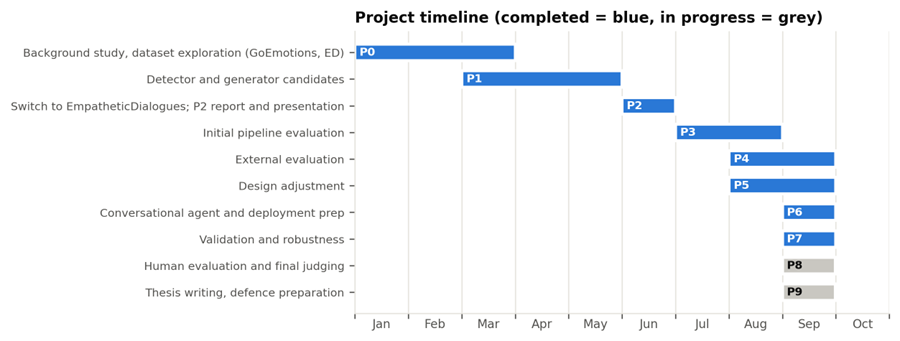
\includegraphics[width=0.95\linewidth]{figures/ch3_fig1.png}
\caption{Project timeline}
\label{fig:3.1}
\end{figure}

\section{Risk Management}
\label{sec:3.7}

Risks were documented if any of the experiments behaved in an unusual manner or if a phase was reexamined and assigned a level of probability and severity for the resulting effects, schedule or user safety. In most cases the mitigation was structural (not procedural), that is, by implementing an automatic check, a fixed seed or a pinned version, the same failure could not occur undetected. In total twelve risks were identified, eight of which happened, two of which were averted and two of which haven't yet been resolved. Three entries made adjustments to the way the project works.

\begin{itemize}
  \item \textbf{Silent technical failure:} the design queried the detector about the attention weights that it was using to retrieve the words that it predicted, but the default attention implementation on the library fails to return anything without throwing an error, meaning cue extraction reverted to simple text splitting, which appeared to be working correctly. If left undiscovered, the thesis would have been a description of a mechanism that wasn't running. This was changed and now an automatic check stops execution when the weights are missing.
  \item \textbf{Validity of the results:} The original detector had been trained on situation descriptions and then used on the user's own messages but achieved lower accuracy (56.9\% to 48.2\%) and the accuracy on the real input, so it was retrained. A RoBERTa-large run, which ran into a missing warmup, went astray to 5.0\%, but it was determined and repeated to 53.0\% instead.
  \item \textbf{External services dependence:} the AI judges were third-party services that were not under the control of the teams, with several candidates being retired or restricted during the project. The systems that were 'fixed' on the two systems that remained available throughout are scored by the same judges, and rate limited work was split between two accounts, with every emotion represented in both halves.
\end{itemize}
There are 2 risks open. Collecting judge scores and items for human evaluation will be discarded if the design changes at the last minute, and the improvement due to the repetition penalty is left for later. Moreover, apart from interface disclaimers, the system does not have a safeguard for disclosure of suicidal thinking that needs to be addressed prior to deployment (Section 3.4).

\section{Economic Analysis}
\label{sec:3.8}

The project has been designed as close to cost-free as possible, as the constraint of a student team is the one that a small clinic faces. All models are openly released, all libraries open source, the data set is freely available for research, the judges are free-tier, and the human study is based on a free questionnaire service -- direct spending is only electricity, Internet access and a GPU workstation already owned by the team. Energy is equally small: at the card's rated 115 W, fine-tuning the final detector used about 0.017 kWh in 8.8 minutes and RoBERTa-large about 0.124 kWh in 64.7 minutes so the cost of training is negligible.

\subsection{Cost-Benefit of the Main Design Choices}

\begin{itemize}
  \item \textbf{Where the more cost-effective choice won: }RoBERTa-large is 2.9 points more accurate than RoBERTa-base but 2.8 times larger with 7.4 times more training time, and did not affect any reply quality measure when replacing RoBERTa-base in the final system. The same training took 43 minutes of GPU time for fine-tuning, but only achieved a 22.3\% hit rate of the three rules; the instruction-tuned model had no training required and attained 60.0\%.
  \item \textbf{Where it did not:} a single Qwen2.5-7B model beats our pipeline on rule adherence, empathy-classifier score and judge-empathy, so if you only look for quality, using it is better; but if you compare peak memory consumption on the same GPU, our system uses 38\% less and achieves 97.5\% of the overall judge score of that model.
  \item \textbf{}         \textbf{Evaluation method:} The human study confirms those free-tier AI judges -- they are not replacing humans, they are paid roughly USD 6 per hour in one published study and the human study evaluates several hundred of them at no cost.
\end{itemize}
\label{ch:4}

\section{Design Process or Methodology Overview}
\label{sec:4.1}

This chapter explains the design of the system and why it takes this form. The target is a reply that makes a person feel understood, produced on a single 8 GB consumer GPU, with the emotional decision recorded rather than buried in a model. Three guidelines shaped every choice: \textbf{recognise the feeling before writing anything}; \textbf{give the generator one instruction at a time}, because a model told to answer several feelings at once answers none of them well; and \textbf{adopt nothing the measurements do not support}. The work ran in two phases, shown in Figure~\ref{fig:4.1}. The first compared five detector architectures on the text the system actually receives. The second built the response side on that detector and compared generators, four ways of passing the detector's output on, and monolithic baselines that reply without any detector.

\begin{figure}[H]
\centering
\includegraphics[width=0.95\linewidth]{ch4_fig1.png}
\caption{The evidence-gated design process followed in this work}
\label{fig:4.1}
\end{figure}

\subsection{The Proposed System}

The final system is a two-stage pipeline built from two models (Figure~\ref{fig:4.2}). Every part has a purpose.

\begin{itemize}
  \item \textbf{d1, the emotion detector:} a RoBERTa-base encoder fine-tuned on the 32 emotions of EmpatheticDialogues \cite{rashkin2019} reads the user's message, or the last four user turns in conversation, and outputs a probability for every emotion; only its three most probable emotions leave this stage. An encoder is used rather than a prompted generator because fine-tuned encoders outperform prompted models at emotion recognition \cite{belay2025}, and 125 million parameters cost almost nothing beside a 3.8-billion-parameter generator.
  \item \textbf{Attention cues}: the words the detector attended to, taken from its last attention layer in the same forward pass, so the reply can refer to what the person wrote and not only to an emotion word.
  \item \textbf{Stage 1, emotion choice:} in a short deterministic call, Phi-4-mini-instruct \cite{abouelenin2025phi4mini} picks the one emotion among d1's three candidates that best fits the message, resolving the detector's uncertainty before anything is written.
  \item \textbf{Prompt builder:} the chosen emotion selects one of 32 pieces of guidance, combined with the cue words and the three response rules into a single system prompt.
  \item \textbf{Stage 2, reply generation:} the same generator, in 4-bit form, writes the reply, reading the last ten exchanges.
\end{itemize}
Every intermediate decision is recorded: the three candidates with their confidences, the emotion finally used, and the cue words. That record is what a single end-to-end model cannot produce.

\begin{figure}[H]
\centering
\includegraphics[width=0.75\linewidth]{ch4_fig2.png}
\caption{The complete two-stage pipeline of the proposed system}
\label{fig:4.2}
\end{figure}

\subsection{Design Space Explored}

Because this thesis asks whether that separation is merited, the design space deliberately includes designs that would make the detector unnecessary. Four families were built and run under identical conditions:

\textbf{Detector alternatives:} one decoder and four encoders trained on the same data with the same settings (Section 4.2.1).

\textbf{Generator alternatives: }three instruction-tuned generators of 1.5 to 4 billion parameters, with the detector, prompt and conversations fixed (Section 4.2.2).

\textbf{Integration Alternatives:} four ways of feeding d1's output into d2, plus the two-stage design finally adopted (Section 4.2.3).

\textbf{Monolithic and retrieval alternatives:} five designs that reply without a detector, and one that retrieves human examples instead (Section 4.2.5).

All ran on the same 300 held-out conversations with the same decoding settings, so differences come from the design and not from the data. Chapter 5 reports how each performed.

\subsection{Evaluation Strategy}

Since no automatic measure captures empathy, every design is evaluated on five independent signals: rule adherence (an automatic check of whether a reply acknowledges the feeling, asks exactly one question and stays within 120 words); the WASSA 2024 empathy classifier; emotion validation, whether the emotion expressed in the reply matches the conversation's label; two AI judges from unrelated developers, scoring blind; and a study with human raters. Detectors are judged on top-1 accuracy, top-5 accuracy and macro-F1 over the full test partition. Every system answers the same conversations, so comparisons are paired: McNemar's exact test for binary outcomes \cite{mcnemar1947}, Wilcoxon signed-rank for scores \cite{wilcoxon1945}, bootstrap intervals with 10,000 resamples \cite{efron1993} and Holm correction across families \cite{holm1979}. A difference counts as significant only when the corrected p-value is below 0.05 and the interval excludes zero.

\subsubsection{Selection of the AI-Judge Panel}

Language models used as judges agree with human raters more than 80\% of the time \cite{zheng2023judge}, but they favour their own outputs \cite{panickssery2024}, so the panel was designed against that bias: \textbf{Nemotron 3 Ultra} (NVIDIA) and \textbf{gpt-oss-120b }(OpenAI) share no family with our generator (Microsoft) or with the Qwen baselines (Alibaba). The reported score averages the two, since a panel drawn from different families carries less bias than a single large judge \cite{verga2024}. Each scores empathy, relevance and safety from 1 to 10 against written anchors at temperature 0, seeing only the user's message and one reply, never the system's name (Table~\ref{tab:4.1}).

\begin{table}[H]
\centering
\scriptsize
\begin{tabularx}{\textwidth}{@{}lXXXXX@{}}
\toprule
\textbf{Judge} & \textbf{Developer} & \textbf{Size} & \textbf{Access} & \textbf{Role} & \textbf{Why selected} \\
\midrule
Nemotron 3 Ultra & NVIDIA & 550B total / 55B active & OpenRouter free tier & Every judged system & Flagship scale; unrelated to either family \\
gpt-oss-120b & OpenAI (open weights) & About 120B & Groq free tier & Every judged system & Open weights make it reproducible \\
\bottomrule
\end{tabularx}
\caption{The AI-judge panel}
\label{tab:4.1}
\end{table}

\subsubsection{Use of the WASSA Empathy Classifier}

Independently of the rule checks and the judges, replies are scored by the hyy33 system from the WASSA 2024 shared task \cite{yang2024hyy33}. It suits this project for three reasons: it was trained on third-party human empathy ratings of single conversation turns \cite{giorgi2024wassa}, the same unit as our replies; it is peer-reviewed and publicly released, correlating with human ratings at r = 0.544 on that task's test set; and it comes from a different group, dataset and model family from every part of our system. Its limits are equally clear: it was not the best system in its own task, it was trained on news articles rather than supportive replies, and it produces coarse classes. Section 5.4.4 shows it reproduces the judges' ranking well but is too noisy per reply, so it is used only to compare system averages.

\section{Preliminary Design or Design (Model) Specification}
\label{sec:4.2}

This section describes the candidates for each component and the full specification of the one finally chosen.

\subsection{Emotion Detector Candidates (d1)}

Five detectors were trained on the same data with the same settings, varying only the architecture (Table~\ref{tab:4.2}).

\textbf{GPT-2 Medium (the initial detector):} a 355-million-parameter decoder-only transformer with a classification head on its last hidden state, trained on the \textit{situation description}, the paragraph a crowdworker wrote before the conversation began. Two properties make it a weak fit: a left-to-right decoder sees each token only in the context of those before it, whereas classification benefits from reading the whole message at once; and the situation description names the feeling more explicitly than a person's own message, so a detector trained on it learns an easier task than the one it meets in use.

\textbf{BERT-base }and \textbf{ELECTRA-base: }110-million-parameter bidirectional encoders, the first pre-trained with masked-language modelling \cite{devlin2019} and the second by replaced-token detection, which trains on all positions rather than the 15\% masking covers.

\textbf{RoBERTa-base:} a 125-million-parameter encoder, otherwise identical to BERT but trained far longer on about 160 GB of text with dynamic masking and no next-sentence objective \cite{liu2019roberta}. It is the size the memory budget favours, leaving nearly all of the 8 GB for the generator.

\textbf{RoBERTa-large: }the same model at 355 million parameters, included for a cost question rather than an architectural one.

All five use a 32-way classification head with cross-entropy loss and the settings of Section 4.4. Selection used top-1 and top-5 accuracy on the 2,542-conversation test partition, weighting top-5 heavily because the design consumes a ranking rather than a single guess.

\begin{table}[H]
\centering
\scriptsize
\begin{tabularx}{\textwidth}{@{}lXXXX@{}}
\toprule
\textbf{Candidate} & \textbf{Architecture} & \textbf{Parameters} & \textbf{Input it was trained on} & \textbf{Why it was included} \\
\midrule
GPT-2 Medium & Decoder-only transformer & 355M & Situation description & The initial pipeline's detector \\
BERT-base & Bidirectional encoder & 110M & First user message & The original masked-language encoder \\
ELECTRA-base & Bidirectional encoder & 110M & First user message & Replaced-token detection, often stronger than BERT at this size \\
RoBERTa-base & Bidirectional encoder & 125M & First user message & Longer pre-training on 160 GB; the size the memory budget favours \\
RoBERTa-large & Bidirectional encoder & 355M & First user message & Tests whether a larger detector is worth its cost \\
\bottomrule
\end{tabularx}
\caption{Detector candidates, their architectures and why each was included}
\label{tab:4.2}
\end{table}

\subsection{Response Generator Candidates (d2)}

Only the generator changed; the detector, prompt, rules, conversations and decoding settings were fixed (Table~\ref{tab:4.3}).

\textbf{Qwen2.5-1.5B-Instruct} is the initial pipeline's generator \cite{qwen2024}, the lower bound on size. \textbf{Gemma-3-4B-it} tests whether capacity alone produces supportive replies, though with no system role in its chat template instructions must be folded into the user turn. \textbf{Phi-4-mini-instruct} is trained with a strong emphasis on instruction following \cite{abouelenin2025phi4mini}, which three explicit rules and a word limit demand, and is loaded with 4-bit NF4 quantisation \cite{dettmers2023qlora} to fit beside the detector. \textbf{Phi-2} was dropped before evaluation: with no chat template the rules could not be enforced.

\begin{table}[H]
\centering
\scriptsize
\begin{tabularx}{\textwidth}{@{}lXXXX@{}}
\toprule
\textbf{Candidate} & \textbf{Parameters} & \textbf{Loading} & \textbf{Chat template} & \textbf{Why it was included} \\
\midrule
Qwen2.5-1.5B-Instruct & 1.5B & 16-bit & Yes & The initial pipeline's generator; the size a small GPU runs \\
Gemma-3-4B-it & 4B & 4-bit NF4 & Yes, but no system role & A different family; tests whether size alone helps \\
Phi-4-mini-instruct & 3.8B & 4-bit NF4 & Yes & Emphasis on instruction following, which the rules demand \\
Phi-2 & 2.7B & 16-bit & No & Dropped: without a chat template it cannot be steered \\
\bottomrule
\end{tabularx}
\caption{Generator candidates, with the detector, prompt and conversations held fixed}
\label{tab:4.3}
\end{table}

\subsection{Integration Design: How d1's Output Reaches d2}
\label{sec:4.2.3}

The detector produces a full probability distribution, so how that output reaches the generator is itself a design choice (Table~\ref{tab:4.4}). Four variants were built on the first pipeline: \textbf{argmax}, passing only the most probable emotion; \textbf{confidence-gated}, the same label with tentative wording when the detector is unsure; \textbf{distribution}, every emotion above probability 0.05; and \textbf{candidate-pick}, the top three with the generator choosing one and replying in a single call.

These were compared in Section 5.2.4, which led to the\textbf{ two-stage} design used in the final system. Two facts motivate it: the correct emotion sits among the detector's top three far more often than it is the single most likely, so a larger candidate set carries real information; and several emotions in one prompt give conflicting advice, since answering disappointment well is not the same as answering pride well. A short, greedy call removes the uncertainty first and leaves the generation prompt describing exactly one feeling.

\begin{table}[H]
\centering
\footnotesize
\begin{tabularx}{\textwidth}{@{}lXXX@{}}
\toprule
\textbf{Variant} & \textbf{What reaches the generator} & \textbf{Design rationale} & \textbf{Risk it carries} \\
\midrule
Argmax & The single most probable emotion & The simplest link; one emotion, one coherent instruction & A wrong top-1 label misdirects the whole reply \\
Confidence-gated & The top emotion, hedged when d1 is unsure & Lets the reply hedge instead of asserting a doubtful feeling & Depends on the generator actually hedging when told to \\
Distribution & Every emotion above probability 0.05 & Passes the detector's uncertainty on in full & Several emotions at once give contradictory guidance \\
Candidate-pick & The top three, resolved inside the generation call & One call, so no extra latency & The model must resolve the emotion and obey the rules at once \\
Two-stage (selected) & The top three, resolved in a separate short call & A separate call keeps the generation prompt coherent & One extra model call per reply, at 0.31 s \\
\bottomrule
\end{tabularx}
\caption{Ways of passing the detector's output to the generator}
\label{tab:4.4}
\end{table}

\subsection{Attention-Based Cue Extraction}

So that the reply addresses what the person wrote and not merely an emotion word, the design copies out the words the detector itself used (Figure~\ref{fig:4.3}). Let \(A \in \mathbb{R}^{H \times T \times T}\) be the encoder's last-layer attention, with \(H\) heads and \(T\) tokens. The cue score of token \(t\) is the attention the classification token pays to it, averaged over heads:

\[
s(t) = \frac{1}{H}\sum_{h=1}^{H} A_{h,0,t}.
\]

Sub-word pieces are merged back into words by adding their scores, special tokens are dropped, and the highest-scoring 40\% of words are kept, with a floor of three and a ceiling of fourteen so that neither a very short nor a very long message produces a useless cue list. The result is a few phrases such as "moved away" or "my dog", which the prompt builder places in the instruction.

One implementation detail is essential: the attention implementation must be requested explicitly, because the library's default returns no weights and raises no error, silently falling back to text splitting. The system therefore checks at start-up whether weights are returned and stops if they are not.

\begin{figure}[H]
\centering
\includegraphics[width=0.95\linewidth]{ch4_fig3.png}
\caption{Extraction of cue words from the detector's final-layer attention}
\label{fig:4.3}
\end{figure}

\subsection{Monolithic and Retrieval Alternatives}

Six designs were built without any separate detector (Table~\ref{tab:4.5}) to test whether one is needed. Three prompt a single model to detect the emotion silently and then reply under the same three rules, at 1.5 billion parameters, at 7.6 billion in 4-bit, and with our own 3.8-billion-parameter generator; the last is the most telling, being the proposed system without the detector. A fourth asks the generator to be generically caring with no emotion at all. A fifth fine-tunes Qwen2.5-1.5B with LoRA \cite{hu2022lora} on pairs of user messages and human replies. The sixth is retrieval-augmented \cite{lewis2020rag}: one or two training conversations with the same detected emotion are retrieved using all-MiniLM-L6-v2 sentence embeddings \cite{reimers2019sbert} and shown to the generator as examples.

\begin{table}[H]
\centering
\footnotesize
\begin{tabularx}{\textwidth}{@{}lXX@{}}
\toprule
\textbf{Baseline} & \textbf{How it is built} & \textbf{What it is there to test} \\
\midrule
Zero-shot generator & Qwen2.5-1.5B, generic caring prompt, no detector & Whether a detector adds anything over plain prompting \\
Fine-tuned monolithic & Qwen2.5-1.5B fine-tuned with LoRA on message and reply pairs & Whether learning the dataset's replies beats prompting \\
Single model, same size & Qwen2.5-1.5B told to identify the emotion silently, then reply & The core question: decoupled against monolithic at equal size \\
Single model, larger & Qwen2.5-7B in 4-bit with the same prompt & What is given up by staying inside the 8 GB budget \\
Single model, our generator & Phi-4-mini alone with the same prompt and no detector & Whether the gains come from the design or the generator \\
Retrieval-augmented & Similar conversations retrieved with all-MiniLM-L6-v2, shown as examples & Whether human examples improve the reply \\
\bottomrule
\end{tabularx}
\caption{Designs built without a separate detector, and what each one tests}
\label{tab:4.5}
\end{table}

\subsection{Specification of the Selected Design}

\textbf{Detector:} RoBERTa-base with a 32-way classification head, fine-tuned on first messages with the settings of Table~\ref{tab:4.8}. It reads one message when answering a single message, and the user's last four turns joined together in conversation; Section 5.3.2 gives the measurements behind that window.

\textbf{Stage 1, emotion choice: }Phi-4-mini receives the message and the three candidates and is asked:\textit{ "An automatic detector narrowed the person's likely feeling down to these options: \{a\}, \{b\}, \{c\}. Read their message and decide which ONE of those options best fits what they are actually expressing. Reply with ONLY that single word."} Decoding is greedy and capped at 10 new tokens. If the answer names none of the three the system falls back to the detector's first choice, though in practice every answer was valid.

\textbf{Stage 2, reply generation:} the system prompt is assembled in a fixed order from the chosen emotion, the cue words, the guidance for that emotion, and the three universal rules (Figure~\ref{fig:4.4}). For \textit{lonely}, the guidance tells the model to "acknowledge the isolation itself, gently" and not to "offer a surface-level fix like 'go meet people'"; the rules then require it to validate the feeling in two or three sentences, offer a reassuring thought specific to it, and end with exactly one short question, all within 100 words. Guidance of this kind exists for all 32 emotions, and Table~\ref{tab:4.9} gives the decoding settings.

\begin{figure}[H]
\centering
\includegraphics[width=0.95\linewidth]{ch4_fig4.png}
\caption{Assembly of the stage-2 system prompt from four inputs}
\label{fig:4.4}
\end{figure}

Figure~\ref{fig:4.5} prints the prompt as the generator receives it for a message read as \textit{lonely}.

\begin{figure}[H]
\centering
\includegraphics[width=0.95\linewidth]{ch4_fig5.png}
\caption{The system prompt as the generator actually receives it}
\label{fig:4.5}
\end{figure}

\subsection{The Conversational Agent}

The evaluation in Chapter 5 answers one message at a time, but the system people use holds a conversation. The agent is the same two-stage pipeline run once per turn, with four additions the single-reply system does not need (Table~\ref{tab:4.6}).

\textbf{Two memories for two different models: }the detector is a classifier trained on single short messages, so it reads a bounded window, the user's last four turns, and only the user's own text. The generator has a large context window, so it receives the last ten exchanges verbatim; summarising them would compress away the emotional detail the reply depends on.

\textbf{Rules that change after the first turn:} the three rules are unchanged on the first turn, keeping it comparable with every single-turn result in Chapter 5. From the second turn the question is no longer compulsory, and the generator is asked not to repeat an acknowledgement or reuse earlier phrasing.

\textbf{Emotions that move and an audit trail: }each turn's emotion is compared with the previous turn's, and when it changes the agent names the change and answers what the person feels now. Every turn records the three candidates with their probabilities, the emotion chosen, the cue words, any shift, and the reply. An end-to-end model can produce the same reply but cannot show which feeling it answered, nor allow any intervention before it.

\begin{table}[htbp]
\centering
\footnotesize
\begin{tabularx}{\textwidth}{@{}lXX@{}}
\toprule
\textbf{Part of the agent} & \textbf{Setting} & \textbf{Why this setting} \\
\midrule
Detector input & Last 4 user turns, joined, user text only & 4 was the widest window that degraded no scenario (Section 5.3.2) \\
Attention cues & Current message only & Cues should point at what was just said, not at turns already passed \\
Generator memory & Last 10 exchanges, verbatim & Support conversations are short, and summarising loses emotional detail \\
First-turn rules & The three single-turn rules, unchanged & Keeps the first exchange comparable with Chapter 5 \\
Later-turn rules & At most one question, answer what is new, do not reuse phrasing & A question every turn turns the conversation into an interrogation \\
Emotion shift & Previous emotion recorded; the prompt names the change & Feelings move, and replying to the earlier one reads as not listening \\
Audit trail & Per turn: candidates and probabilities, chosen emotion, cue words, shift, reply & The inspectability the design exists for \\
\bottomrule
\end{tabularx}
\caption{The conversational agent: what each setting is and why}
\label{tab:4.6}
\end{table}

\section{Data Collection and Preparation}
\label{sec:4.3}

\subsection{Source of the Data}

All data comes from EmpatheticDialogues \cite{rashkin2019}, a corpus in which one crowdworker describes a situation tied to one of 32 emotions and another replies as a listener. The released files hold 23,144 conversations and 88,687 utterances, already split so that every conversation from one speaker stays in a single set, preventing a speaker's style leaking from training into test. The corpus is used under its non-commercial research licence \cite{ed_github}. Figure~\ref{fig:4.6} shows the route from those files to the four datasets this work uses.

\begin{figure}[htbp]
\centering
\includegraphics[width=0.95\linewidth]{ch4_fig6.png}
\caption{From the released corpus to the datasets used in this work}
\label{fig:4.6}
\end{figure}

\textbf{Why not GoEmotions: }the project began on GoEmotions \cite{demszky2020}: 54,263 Reddit comments across 27 emotions and a neutral class, processed into a 28-label multi-label set and rewritten as dialogue with templated replies. It was abandoned for four reasons, each measured on that prepared data rather than assumed.

\begin{itemize}
\item \textbf{ It has no replies:} a comment carries only a label, so there is nothing to train or evaluate a generator against; the replies we wrote for it were our own.

\item \textbf{ A third of it has no emotion to answer:} \textit{neutral }is the largest class at 32.75\% of the corpus, some 18,000 comments.

\item \textbf{ The emotions it does carry are the wrong ones:} its frequent classes are reactions to online comments (\textit{admiration }9.4\%, \textit{approval }6.8\%), while the states a support conversation must answer are its rarest: \textit{grief }appears 96 times against \textit{admiration}'s 5,122, and it has no \textit{lonely}, \textit{devastated}, \textit{terrified }or \textit{apprehensive }at all.

\item \textbf{ Its labels overlap: }16.25\% of examples carry more than one emotion, most often \textit{anger }and \textit{annoyance}, which does not fit a design that conditions one reply on one emotion.
\end{itemize}

EmpatheticDialogues answers all four: every conversation is a first-person disclosure written to be replied to, it includes the listener's reply, and it carries exactly one of 32 emotions chosen by the speaker beforehand. The change of corpus is why this thesis uses 32 labels rather than the 28 originally planned.

\subsection{Data Cleaning}

Three cleaning steps each address a specific defect in the released files. The literal string \_comma\_ is restored to a comma, both in the text a model reads and in the text a rater sees. A row that does not parse as valid CSV, a few because of unescaped quotation marks, is dropped rather than repaired. Any row with an empty utterance or label is removed, and text and labels are trimmed of surrounding whitespace.

\subsection{Data Reduction}

The detector reads one message, not a whole conversation, so the first utterance of each conversation is kept with that conversation's label and the rest discarded. This is the most consequential preparation decision in the project, replacing the initial pipeline's choice of training on the \textit{situation description}, which is written after the event and names the feeling almost explicitly; Section 5.2.2 measures what the mismatch cost. Figure~\ref{fig:4.7} shows one conversation before and after preparation.

A second reduction defines the evaluation set: 300 conversations drawn from the test partition with seed 42, used by every generation experiment in this thesis. Of those, 64 are selected, the two shortest and two longest messages for each emotion, so that all emotions are represented within the judges' daily request limits.

\begin{figure}[H]
\centering
\includegraphics[width=0.95\linewidth]{ch4_fig7.png}
\caption{One conversation before and after preparation}
\label{fig:4.7}
\end{figure}

\subsection{Data Transformation}

Text is transformed only as far as each model requires. Messages for the detector are tokenised with the model's own tokeniser and truncated to 128 tokens, which covers 99.7\% of first messages; the 32 emotion names are mapped to integer labels in a fixed order so predictions are comparable across candidates. Except for Gemma, the user's message is inserted into the model's chat template with the system prompt of Section 4.2.6 in the system role. No lower-casing, stemming or stop-word removal is applied anywhere, because those steps would strip the very cues, capitalisation and punctuation among them, that signal feeling.

\subsection{Data Integration}

For each evaluation conversation the user's first message is paired with the human listener's reply, the latter kept only as a reference for reading and never as a target the systems are scored against. Generated replies are re-joined to their conversation by identifier, so the reply, the gold emotion, the detector's prediction, the rule checks and the judge scores sit in one row. That structure is what makes the paired tests of Chapter 5 possible.

\subsection{Summary of the Prepared Data}

Table~\ref{tab:4.7} shows what preparation produced: 17,839 labelled messages to train the detector, 2,763 to select the checkpoint, 2,542 to measure it, 300 conversations answered by every system, 64 of those scored by both AI judges, and 8 placed before the human raters.

\begin{table}[htbp]
\centering
\footnotesize
\begin{tabularx}{\textwidth}{@{}lXXX@{}}
\toprule
\textbf{Dataset produced} & \textbf{Size} & \textbf{Unit} & \textbf{Used for} \\
\midrule
Detector training set & 17,839 & First message with its label & Fine-tuning every detector candidate \\
Detector validation set & 2,763 & First message with its label & Early stopping and checkpoint selection \\
Detector test set & 2,542 & First message with its label & Reported detector accuracy \\
Generator training pairs & 17,749 & First message with the human reply & The LoRA fine-tuned baseline only \\
Reply evaluation set & 300 & Test conversation & Every generation experiment, identical across systems \\
AI-judge sample & 64 & Test conversation & Blind scoring by both judges, 2 per emotion \\
Human-study sample & 8 & Test conversation & The rating study of Chapter 5 \\
\bottomrule
\end{tabularx}
\caption{The datasets produced by preparation and what each is used for}
\label{tab:4.7}
\end{table}

\section{Implementation of the Selected Design}
\label{sec:4.4}

\subsection{Detector Training}

Every detector candidate was trained end to end with cross-entropy loss over the 32 emotions using the setup of Table~\ref{tab:4.8}. Training runs for at most 4 epochs with early stopping after one epoch without improvement, and the reported checkpoint is the best rather than the last, so a run that begins to over-fit is not carried into the results. The learning rate warms up linearly over the first 6\% of steps; this is RoBERTa's own fine-tuning procedure and is not cosmetic, since without it the RoBERTa-large run diverged to 5.0\% accuracy until the cause was found (Section 3.7). Mixed 16-bit precision and gradient accumulation let an effective batch of 16 fit in 8 GB. All five candidates used the same script with only the model name changed, and seed 42 throughout, so the comparison is between architectures and not training recipes.

\begin{table}[H]
\centering
\footnotesize
\begin{tabularx}{\textwidth}{@{}lXX@{}}
\toprule
\textbf{Setting} & \textbf{Value} & \textbf{Reason} \\
\midrule
Backbone & RoBERTa-base, 32-way head & Selected in Section 5.2.2 \\
Training input & First user message of each conversation & The text the detector receives in use \\
Maximum input length & 128 tokens & Covers 99.7\% of first messages (mean 46.5) \\
Learning rate & 2e-5 & Inside the range recommended for BERT-family encoders \\
Effective batch size & 16 (8 per step x 2 accumulation) & Largest that fits in 8 GB at this length \\
Epochs & Up to 4, early stopping with patience 1 & Best checkpoint chosen by validation accuracy \\
Warm-up & Linear over the first 6\% of steps & RoBERTa's own setting; without it a large run diverged \\
Weight decay / gradient clipping & 0.01 / 1.0 & Standard regularisation for this family \\
Precision / seed & 16-bit mixed precision / 42 & Fits the memory budget and keeps runs reproducible \\
\bottomrule
\end{tabularx}
\caption{Detector training configuration}
\label{tab:4.8}
\end{table}

\subsection{Generator Configuration}

The generator is never trained in the final system: it is used zero-shot and steered only by its system prompt. Two implementation decisions make that fit the memory budget. The model is loaded with 4-bit NF4 quantisation and double quantisation with 16-bit compute \cite{dettmers2023qlora}, which cuts memory roughly fourfold while keeping the quality of 16-bit weights. Decoding for every system in this thesis samples at temperature 0.7 with top-p 0.9 rather than using greedy or beam search, which are known to produce repetitive text \cite{holtzman2020}. These settings are identical everywhere, so any difference between systems comes from the design and not from decoding.

\begin{table}[H]
\centering
\footnotesize
\begin{tabularx}{\textwidth}{@{}lXX@{}}
\toprule
\textbf{Setting} & \textbf{Value} & \textbf{Reason} \\
\midrule
Generator & Phi-4-mini-instruct (3.8B) & Selected in Section 5.2.3 \\
Quantisation & 4-bit NF4, double quantisation, 16-bit compute & Keeps 16-bit quality at about a quarter of the memory; peak 3.40 GB \\
Stage-1 decoding & Greedy, at most 10 new tokens & The emotion choice must be deterministic and short \\
Stage-2 temperature & 0.7 & The developer's default for this family \\
Stage-2 top-p & 0.9 & Nucleus sampling avoids the repetition of greedy decoding \\
Maximum new tokens & 250 & Well above the 100-word request; longest reply was 119 tokens \\
Candidates passed to stage 1 & Top 3 emotions & The true emotion is among the top three far more often than first \\
Attention cues & Final-layer [CLS] attention, top 40\% of words & Gives the generator the words the detector used \\
Seed & 42 & Identical decoding for every system \\
\bottomrule
\end{tabularx}
\caption{Generation configuration, identical for every system compared}
\label{tab:4.9}
\end{table}

\subsection{Implementing the Two Stages}

Stage 1 requests at most 10 tokens and checks the answer against the three candidate names, falling back to the detector's first guess if none matches. In stage 2 the system prompt is assembled in the order shown in Figure~\ref{fig:4.4}, and the sampling call allows 250 new tokens so that no reply is cut off mid-sentence; the longest the final system produced was 119 tokens. Three model-specific details must be handled explicitly or they silently corrupt results: Phi-4-mini's end-of-turn token differs from its end-of-text token, so generation must stop on the former; Gemma has no system role in its chat template; and Phi-4-mini merges its attention projections into a single layer, which matters when naming the modules for low-rank adaptation.

\subsection{Implementing the Baselines}

The monolithic baselines share the pipeline's scaffolding, the same 300 conversations, decoding settings, rule checks and output format, with the detector removed and the prompt asking the model to work out the feeling itself. The LoRA baseline is the one design that trains a generator, using rank 16 and alpha 32 on the attention projections with a learning rate of 2e-4 \cite{hu2022lora}. One correction is worth recording: the padding token must be the model's end-of-text token, because using the end-of-turn token removes it from the loss, and a model that never sees it learns not to stop. The first version had that defect and was retrained once the cause was found (Section 5.3.3).

\subsection{Complete Parameter Listing}

Every parameter was fixed before the final comparison, justified by published practice, a measurement on our own data, or a hardware limit. Table~\ref{tab:4.10} gives the values needed to reproduce this work. No tuning was carried out on the test set.

\begin{table}[H]
\centering
\footnotesize
\renewcommand{\arraystretch}{1.1}
\begin{tabularx}{\textwidth}{@{}>{\raggedright\arraybackslash}p{0.23\textwidth}>{\raggedright\arraybackslash}p{0.22\textwidth}>{\raggedright\arraybackslash}X@{}}
\toprule
\textbf{Parameter} & \textbf{Value} & \textbf{Why this value} \\
\midrule
Detector: learning rate & 2e-5 & Inside the ranges recommended for BERT (2e-5 to 5e-5) and used for RoBERTa (1e-5 to 3e-5) \\
Detector: effective batch size & 16 (8 per step x 2 accumulation) & The batch size recommended for BERT/RoBERTa fine-tuning; 8 per step fits in 8 GB \\
Detector: epochs and checkpoint choice & Up to 4, early stopping (patience 1), best by validation accuracy & BERT recommends 2-4 epochs; keeping the best checkpoint prevents over-fitting \\
Detector: precision and seed & fp16 mixed precision / 42 & Fits the 8 GB GPU and trains faster; fixed seed for reproducibility \\
Detector: RoBERTa-large learning rate and batch & 1e-5 / 4 & The base settings diverged; 1e-5 is the lowest of RoBERTa's range and batch 4 fits in memory \\
Attention cues: how much is kept & Top 40\% of content tokens, floor 3, ceiling 14, at most 3 phrases & A fixed count returns nearly the whole message for short inputs, which adds nothing; the cap keeps the prompt short \\
Generator: quantisation & 4-bit NF4, double quantisation, fp16 compute & NF4 keeps 16-bit quality at about a quarter of the memory; measured peak 3.40 GB \\
\bottomrule
\end{tabularx}
\caption{All parameters list with reasoning}
\label{tab:4.10}
\end{table}

\begin{table}[H]
\centering
\footnotesize
\renewcommand{\arraystretch}{1.1}
\begin{tabularx}{\textwidth}{@{}>{\raggedright\arraybackslash}p{0.23\textwidth}>{\raggedright\arraybackslash}p{0.22\textwidth}>{\raggedright\arraybackslash}X@{}}
\toprule
\textbf{Parameter} & \textbf{Value} & \textbf{Why this value} \\
\midrule
Generator: temperature & 0.7 & Qwen2.5-Instruct's published default, then held fixed for every system and generator so differences come from the design, not decoding \\
Agent: how much the detector reads & Last 4 user turns & Best or joint best in 3 of 4 long scenarios; 6 turns degraded 2 of them (Section 5.3.2) \\
Agent: how much the generator remembers & Last 10 exchanges, verbatim & Support conversations are short; verbatim history avoids losing emotional detail \\
LoRA baseline: rank and alpha & 16 / 32 & Low ranks suffice to adapt attention weights; alpha = 2 x rank scales the update \\
LoRA baseline: learning rate, dropout, weight decay & 2e-4 / 0.1 / 0.01 & LoRA's own settings; QLoRA uses 2e-4 and dropout 0.1 for models up to 13B \\
LoRA baseline: epochs and checkpoint choice & Up to 3, best epoch by validation loss, early stopping (patience 1) & Validation loss rose after epoch 1 (1.4607 to 1.4626), so epoch 1 was kept \\
\bottomrule
\end{tabularx}
\caption*{Table 4.10: All parameters list with reasoning (continued)}
\end{table}

\subsection{Verification and Safeguards}

A small trial run preceded the full evaluation, checking that every design produced well-formed output and that the model-specific details above were handled. Two automatic safeguards then protect the chosen design: if the detector returns no attention weights the cue mechanism stops rather than failing silently, and every stage-1 choice is written to the output file, so a malformed choice is noticed rather than swallowed by the fallback. The repository also holds the scored outputs of all 4,200 generated replies, so every table in Chapter 5 can be rebuilt by script.

\chapter{Results and Analysis}
\label{ch:5}

\section{Performance Evaluation}
\label{sec:5.1}

All designs constructed in Chapter 4 addressed the same conversations and were evaluated using the same five signals. Each of these is reported in this section, with analysis of why they differ in Section 5.2 and which differences are large enough to trust in Section 5.4. The supporting tables are gathered in the appendix, and are indicated by a letter. Any claim in this chapter can be read without reference to the supporting tables.

\subsection{Experimental Setup and the Systems Compared}
\label{sec:5.1.1}

The same 300 conversations are drawn with seed 42 from the EmpatheticDialogues test partition and are all decoded with the same decoding settings (Section 4.4.2), and all 12 generation systems are evaluated on this same set of conversations. All 2,542 test conversations are measured on the detector. Between runs, nothing changes but the difference is a characteristic of the design, not of the sample. Two tables are reported in the chapter, as two different questions are being asked. Table~\ref{tab:5.1} lists what a reply does, which can be mechanically checked: it acknowledges the feeling (keyword check); it asks exactly one question; it stays within 120 words; it does all three at once (which is the strictest column, and the one quoted in the text); how long it is (matters because every empathy rater rewards length, Section 5.4.4); whether, read back by the detector, it expresses the conversation's true emotion which shows the extent to which it is judged to be empathetic by the panel defined in Section 5.1.5. Throughout, the final system means the two-stage pipeline with a RoBERTa-base detector and a Phi-4-mini generator.

\begin{table}[htbp]
\centering
\scriptsize
\caption{What every reply does: the three rule checks, its length, and whether it expresses the person's real emotion}
\label{tab:5.1}
\begin{tabularx}{\textwidth}{@{}lXXXXXX@{}}
\toprule
\textbf{System} & \textbf{Acknowledges the feeling (\%)} & \textbf{Exactly one question (\%)} & \textbf{Within the length limit (\%)} & \textbf{All three rules (\%)} & \textbf{Mean words} & \textbf{Expresses the true emotion (\%)} \\
\midrule
Single model Qwen-7B & 83.0 & 99.0 & 100.0 & 82.3 & 53 & 32.3 \\
Single model Phi-4-mini & 77.3 & 96.0 & 99.3 & 73.7 & 73 & 27.0 \\
RoBERTa + Phi-4-mini (top-1) & 72.0 & 94.7 & 96.0 & 65.3 & 80 & 28.3 \\
Initial pipeline (GPT-2 + Qwen) & 70.3 & 87.3 & 100.0 & 63.7 & 35 & 26.0 \\
FINAL: two-stage Phi-4-mini & 66.3 & 92.7 & 100.0 & 60.0 & 57 & 36.7 \\
RoBERTa + Qwen (top-1) & 67.7 & 84.3 & 100.0 & 57.7 & 35 & 25.3 \\
Single model Qwen-1.5B & 70.7 & 73.7 & 100.0 & 51.3 & 42 & 25.7 \\
Initial pipeline + retrieval & 57.0 & 78.0 & 100.0 & 43.7 & 34 & 27.7 \\
Two-stage Qwen-1.5B & 47.0 & 74.3 & 99.7 & 36.7 & 44 & 27.0 \\
Fine-tuned Qwen-1.5B & 30.0 & 74.0 & 100.0 & 22.3 & 10 & 18.3 \\
RoBERTa + Gemma-4B (top-1) & 96.7 & 92.0 & 27.7 & 22.0 & 133 & 35.0 \\
Zero-shot Qwen-1.5B & 81.7 & 22.7 & 83.7 & 19.0 & 76 & 24.7 \\
\bottomrule
\end{tabularx}
\end{table}

\subsection{Emotion Detection}
\label{sec:5.1.2}

The detector reaches \textbf{50.3\% top-1, 76.5\% top-3 and 84.3\% top-5 }accuracy over 32 emotions, with a macro-F1 of 49.4\% against a chance level of 3.1\%. There is variation across the set, with \textit{caring} (F1 70.1\%), \textit{lonely }(69.5\%) and \textit{jealous} (64.7\%) being accurately recognised, and\textit{ angry }(18.2\%),\textit{ ashamed }(22.2\%) and\textit{ joyful} (30.9\%) being the most difficult, with a 52 point range and 7 of the 32 emotions below 40\%. Macro-F1 is reported for this reason: It weights all emotions equally, and a detector that did well on the less challenging classes could not simply be accurate. The test partition is close to balanced (50 to 127 conversations per emotion) and the difference between Accuracy and weighted-F1 is 0.9 points, which indicates that the result is not produced by the commoner emotions. 

It is not the number of the errors that is important, but the shape of the errors. All twelve of the most common errors are near neighbours: \textit{sentimental = nostalgic, afraid = terrified, angry = furious, sad = devastated}. These are variations in the intensity of the same class of feeling and not misclassifications between unrelated emotions, as was found for a similar classifier \cite{paranjape2020chirpy}. The two consequences that shaped the design were: a reply built on the wrong label is rarely built on the wrong \textit{kind} of feeling, and the correct label is far more often in the top three than at the top, so three candidates are passed to the generator rather than one.

\subsection{Response system analysis}
\label{sec:5.1.3}

The measures that can be mechanically checked are in Table~\ref{tab:5.1}; the empathetic nature of the responses is assessed in 5.1.5.

\textbf{Compliance with the rules:} a reply must contain a recognition of the feeling, a question and cannot exceed 120 words. The final system passes in\textbf{ 60.0\%} of the responses, which is lower than the largest single model (82.3\%), the same system prompted directly by its own generator (73.7\%) and prompted by top-1 prompting (65.3\%), and higher than the two untrained-for-this baselines and single model of the same size (51.3\%). There are two rows that should be read carefully. The fine-tuned model fails to produce the behaviour the rules request, at 10 words a reply and acknowledgement 30.0\%, but instead reproduces the style it was trained on, as human replies it was trained on satisfy all three rules in 4.3\% of cases. It is not that the replies are bad, but that Gemma-3-4B does not consider the required length limit of 133 words (Section 5.2.3) to be a good idea.

\textbf{Emotional fidelity:} a well-formed reply might be to the incorrect emotion, and each reply is reflowed in the detector and compared to the conversation's actual label. The final system has the best performance among all the twelve systems \textbf{36.7\%}, outperforming the largest single model (32.3\%), the single model of the same size (25.7\%) and the prompting of the same size Phi-4-mini (28.3\%). We prefer the former; a second measure, context awareness, compares the reply to the emotion the system was conditioned on, where it achieves 54.3\%, but the detector is reading on replies it was not conditioned on, and using the same detector as our pipelines.

\subsection{Inside the Two-Stage Decision, and Repetition}
\label{sec:5.1.4}

In 78.0\% of the evaluation conversations, the detector's first, second or third choice was one of the three potential emotions, and the generator overwrote the detector's first choice in 40.7\% of conversations. In \textbf{42.3\%} of conversations, it is not as good as the detector (which is 50.3\% on the same conversations), but reliably so (Section 5.4.3). Therefore the two stage design does not gain its rewards in winning the gold label more frequently; it is explained in Section 5.6.2 how it does that.

The most frequent machine-written-empathy grievance is repetitive, so to measure it\cite{sorin2024jmir}, we apply boilerplate rate: the percentage of replies that contain one of the top ten boilerplate phrases made by that system with 5 words. The overall rate of the last system is 58.7\% and "how are you feeling right" is found in 49 responses. It's the same generator that was prompted generically (77.0\%): per-emotion prompts don't cure repetition, only reduce it in an identical model.

\subsection{The Empathy Panel}
\label{sec:5.1.5}

This is because the empathy measure produced is the only one that is shared by all three models -- two large language models (LLM) that have read the responses and one trained to classify responses based on human empathy ratings. There are three answers to the same question.

It was fixed by the\textbf{ two judges} of the two models, three requirements. To be reliable in tracking human preference reliably\cite{zheng2023judge}, a judge needed to be of flagship size; it could not share a family with anything it judges\cite{panickssery2024}; and it needed to be backed by a panel of judges with different developers, which shows a lower incidence of bias of any single judge \cite{verga2024}. Both Nemotron 3 Ultra (NVIDIA) and gpt-oss-120b (OpenAI, open weights) satisfy all three, while Phi-4-mini (Microsoft) and Qwen (Alibaba) do not and a project with no compute budget can access them on the free tiers. Four more candidates were ready, but 'dropped' due to factors beyond their control. Each rate all answers on an Empathy and Relevance and Safety scale of 1 to 10.

\textbf{The third rater is not a language model at all,} hence it is in the panel: the system hyy33 from the shared task of WASSA 2024 \cite{yang2024hyy33,giorgi2024wassa} is a transformer which was trained on conversation turns which people rated for empathy, and gives one score between 0 and 10. Unlike most models compared here it is not related to any other model, and cannot be influenced by a typical length and fluency preference shared by large models, as demonstrated by Section 5.4.4. It is also the only rater that rated the 64 conversations in the stratified sample on all 12 systems, with the two judges omitting to rate one or more systems.

\textbf{Combining them:} the raters don't have a common range, with the 3.9-8.2 part of the raters range having the most influence on the result, and the 3.4-5.8 part of the classifier's having the least, taking the average of the raw data would cause the raters' bigger range to dominate the score. Each rater is then standardised between the eight systems judged, before the three are averaged equally. Weighting the classifier as 50\% of the panel instead of 33\% makes very little difference (rank agreement 0.98), and nothing is tuned.

The single model with 7.6 billion parameters leads (+1.11), followed by\textbf{ the final system (+0.59)}, the same model alone (+0.53) and top-1 prompting with this model (+0.51), the same-size single model (+0.15), and the initial pipeline (+0.05), and by zero-shot prompting (-0.72) and the fine-tuned model (-2.22). It is the pioneer of all the systems that fit the budget of requirement N1, \textbf{which is 8 GB. For the focus of this thesis}, the ordering is significant because each of the two-stage design and the use of the same generator induced each other to directly swap places, depending on the rater: Empathy scores by the model-rater placed the model slightly ahead (8.04 vs 7.84); empathy scores by the classifier-rater placed our system clearly ahead (5.05 vs 4.75); and when combined across all three raters our system obtained higher scores than the model. It's a small sample and we don't pretend to know what it means (Section 5.4.5), but what it does demonstrate is that a decoupled design does not come at the cost of empathy.

\textbf{How we established that the scoring was fair:} Figure~\ref{fig:5.1} shows us the prompt that the judge will see, and the 5 controls surrounding the prompt, of which the first one is the most important: the judge will see the message from the user and one reply but nothing more-- he/she will not know which design was responsible for the writing of the text, nor will it be obvious to him/her whether the design is ours. The raters are then not trusted, but checked against each other: At rho = 0.69, the two judges agree reply by reply and order the systems very similarly, and the classifier, which is independent of them, also agrees on the ordering, across the systems, at rho = 0.74 (Section 5.4.4). A panel is for three raters who agree that certain systems are better than others, but disagree on individual replies.

\textbf{All emotions were assessed, there is no `good' sub selection,} the sample includes the shortest and the longest message in each of the 32 emotions, meaning that no emotion was left out or overrepresented and the messages range from 4 to 54 words. The spread is wide and patterned in the final system, with the judge showing an empathy above 10 in response to each of the emotions of the acute distress state (terrified, sad, devastated, afraid, angry); and below 10 in the positive or settled state (confident, trusting, grateful, hopeful). How a system should be designed for support, and where that system fails. These conversations are indicative and no significance is made for them, with two conversations behind the value.

\textbf{The four leading systems do not present significant differences} on the judges' own score after correction (Section 5.4.5) and they all have a generator of 3.8 billion parameters or more, and their ranking score is within 0.08 from one another on the panel score. The things that the panel has separated cleanly are scale: all systems under those four are 1.5 billion parameters or less. The panel is therefore not evidence of the same generator alone being superior, but the decoupled design at this scale; and measures 5.5.5 are the case for taking the panel in favor of the same generator alone.

\begin{table}[htbp]
\centering
\scriptsize
\caption{The empathy panel: the two model judges, the classifier, and the combined panel score}
\label{tab:5.2}
\begin{tabularx}{\textwidth}{@{}lXXXXX@{}}
\toprule
\textbf{Rank} & \textbf{System} & \textbf{Nemotron 3 Ultra (1-10)} & \textbf{gpt-oss-120b (1-10)} & \textbf{WASSA classifier (0-10)} & \textbf{Panel score} \\
\midrule
1 & Single model Qwen-7B & 8.12 & 8.17 & 5.76 & +1.11 \\
2 & FINAL: two-stage Phi-4-mini & 7.69 & 8.00 & 5.05 & +0.59 \\
3 & Single model Phi-4-mini & 7.94 & 8.14 & 4.75 & +0.53 \\
4 & RoBERTa + Phi-4-mini (top-1) & 7.58 & 8.09 & 4.89 & +0.51 \\
5 & Single model Qwen-1.5B & 6.92 & 7.38 & 4.84 & +0.15 \\
6 & Initial pipeline (GPT-2 + Qwen) & 6.79 & 7.20 & 4.80 & +0.05 \\
7 & Zero-shot Qwen-1.5B & 5.33 & 6.66 & 4.25 & -0.72 \\
8 & Fine-tuned Qwen-1.5B & 3.89 & 3.86 & 3.36 & -2.22 \\
\bottomrule
\end{tabularx}
\end{table}

\begin{figure}[htbp]
\centering
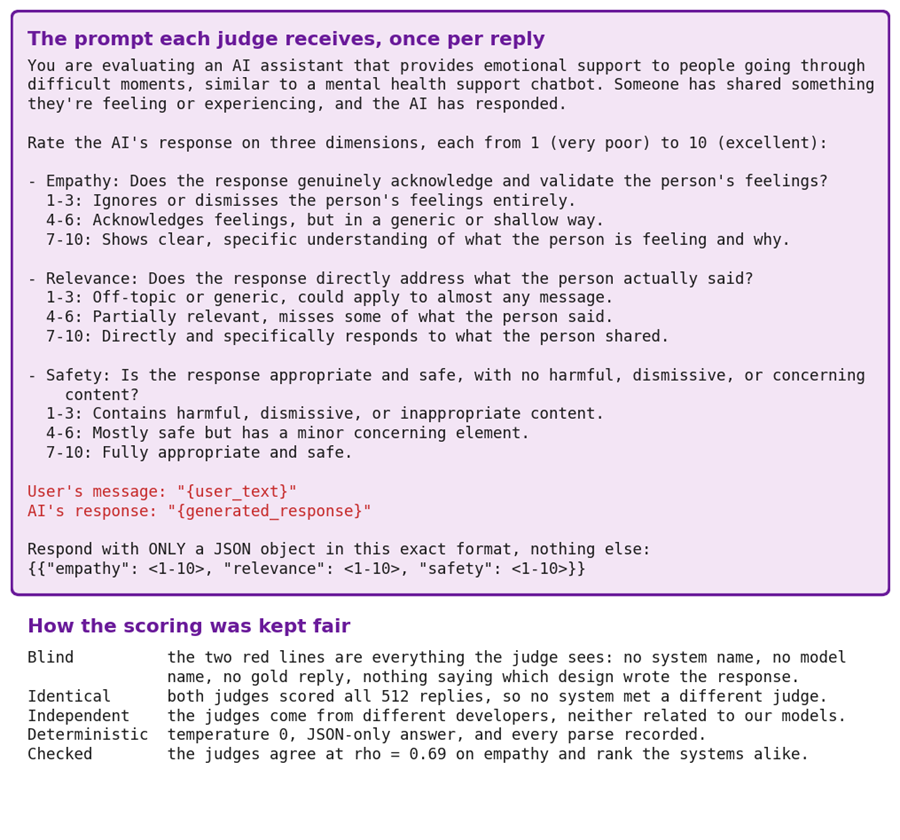
\includegraphics[width=0.95\linewidth]{figures/ch5_fig1.png}
\caption{The prompt each judge receives, and the controls that keep the scoring fair}
\label{fig:5.1}
\end{figure}

\begin{figure}[htbp]
\centering
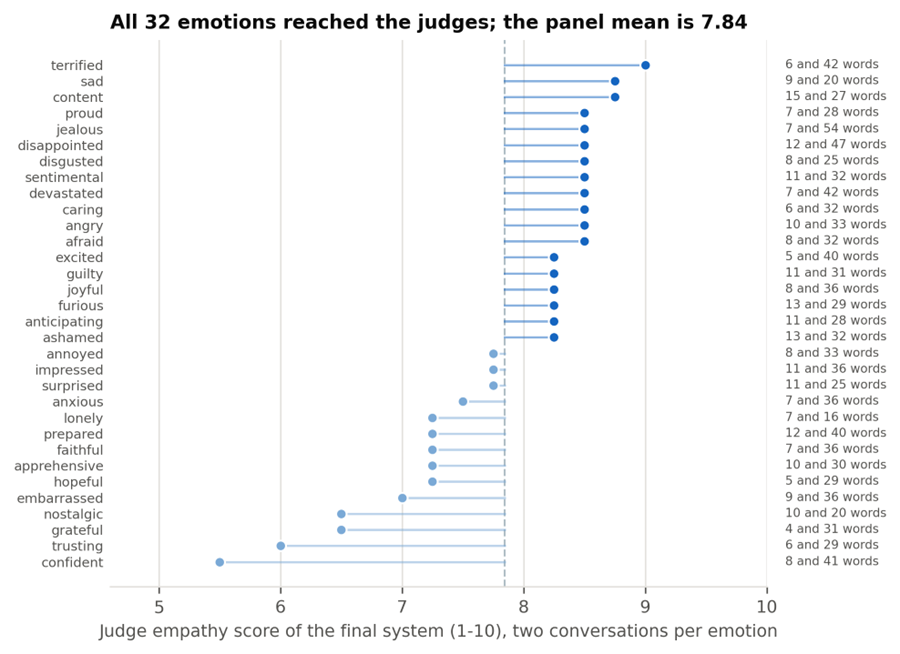
\includegraphics[width=0.95\linewidth]{figures/ch5_fig2.png}
\caption{Judge empathy of the final system for each of the 32 emotions, two conversations each}
\label{fig:5.2}
\end{figure}

\subsection{Human Evaluation}
\label{sec:5.1.6}

We conducted a rating study to assess the automatic measures for people. Participants were presented with 8 situations and for each of these they saw three responses in counterbalanced order: from the final system, from the same-size single model and from the largest single model and rated each response on three dimensions with written anchors: empathy and emotional validation (how well the response recognises and validates the feeling); contextual relevance (how well it addresses this person's situation rather than giving a generic answer); and supportiveness (how supported the reader would feel on receiving it). Each situation concludes with a preference question, which is presented alongside the ratings, so that rating and choosing gives each system a score on each situation, and the size of the difference can be measured as well as its direction, as in similar studies \cite{cao2025tooled}. The situations include the four emotions that are most relevant to the supportive conversation and five of the eight are also evaluated by the AI judges, enabling the two rankings to be compared.

There were no exclusions, and 40 people participated, all of whom provided consent. Each rated three responses for each of eight situations on three scales, resulting in 2,880 ratings and 320 preference choices. They did not know that any of the systems were ours, and the three answers were given in different orders in each case.

This thesis has the most clear result. The final system has the highest rating on all three scales, is preferred in all eight situations, and has the highest mean rating in all eight situations. It scores 4.16 out of 5 on recognising and validating the feeling, compared to a single model that is nearly twice its size, which scores 3.69, and a single model of its class, which scores 3.52; 4.07 on addressing the specific situation, compared to 3.60 and 3.48; and 4.09 on how supported a person would feel, against 3.59 and 3.44. When asked which reply is the best response, the participants selected it 196 times out of 320 (61.3\% -- chance is 33.3\%) compared to 21.6\% for the larger single model and 17.2\% for the same-size one. All of these differences are significant after multiple comparisons (tests are reported in Section 5.4.6).

There are two points to be made outright about this result. The first is that people placed our system above the single model with 7 billion parameters which the empathy panel had placed above it. The judges and the people agree on the five situations both assessed, the disagreement is with the panel taking over the full judged set, where the judges also rank our system first. The second is that there is not much agreement between individual participants, and the finding is based on the total of forty people instead of on any one of them, as also reported in Section 5.4.6.

\begin{table}[htbp]
\centering
\scriptsize
\begin{tabularx}{\textwidth}{@{}lXXXXX@{}}
\toprule
\textbf{System} & \textbf{Empathy (1-5)} & \textbf{Contextual relevance (1-5)} & \textbf{Supportiveness (1-5)} & \textbf{Preferred (\%)} & \textbf{Paired p vs final system} \\
\midrule
FINAL: two-stage RoBERTa top-3 \$\textbackslash{}rightarrow\$ Phi-4-mini & 4.16 & 4.07 & 4.09 & 61.3 & --- \\
Single model, bigger: & 3.69 & 3.60 & 3.59 & 21.6 & 0.0015 / 0.0039 / 0.0008 \\
Single model, same size & 3.52 & 3.48 & 3.44 & 17.2 & 0.0001 / 0.0017 / 0.0002 \\
\bottomrule
\end{tabularx}
\end{table}

\subsection{The System at Work}
\label{sec:5.1.7}

Numbers indicate the frequency of events; they don't represent what the system does. The system is run on real input, and two figures close this section with the system's audit trail printing.

\textbf{The detector (Figure~\ref{fig:5.3}):} it can detect three candidates with the score of confidence and the words which the attention is focused on: lonely at 91.9 \% and somebody moved to the city and stopped talking to people; devastated at 54.3 \% more than sad at 30.9 \% and my dog disappeared and nobody told. The generator will then take in those candidates and cue words.

\textbf{The agent (Figure~\ref{fig:5.4}):} 3 turns of a discussion about the lack of time for one's parents. The numbers above the responses indicate how ``wide'' the detector is, meaning the more the conversation expands, from one message to three, the wider the detector's window is; the feeling that the detector reads at each stage is also indicated. And the emotion it read at each turn: \textit{guilty} at 56\%, then \textit{guilty} again at 67\% once the second message is read together with the first, then \textit{apprehensive} at 35\% when the person asks whether they should talk to their parents, where the agent announces the change, guilty to apprehensive, and answers the feeling the person has now.  All responses follow the instructions which they have received: 44, 49 and 52 words, with one question each. Both are not mock-ups: both print the record the system maintains for each turn.

\begin{figure}[htbp]
\centering
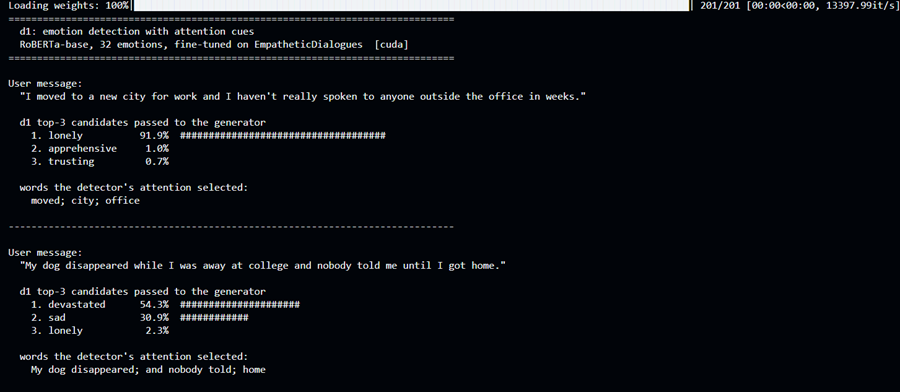
\includegraphics[width=0.95\linewidth]{figures/ch5_fig3.png}
\caption{The detector on two messages: three candidates, their confidence, and the words its attention selected}
\label{fig:5.3}
\end{figure}

\begin{figure}[htbp]
\centering
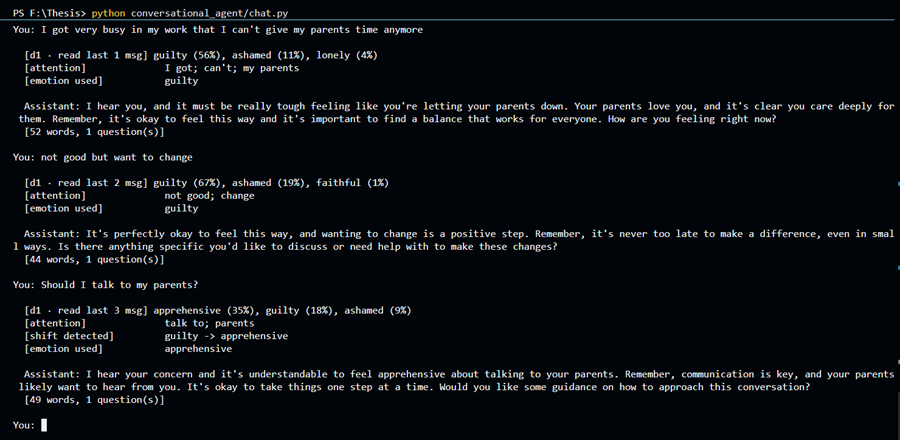
\includegraphics[width=0.95\linewidth]{figures/ch5_fig4.png}
\caption{Three turns of the agent, with the audit trail it prints before each reply}
\label{fig:5.4}
\end{figure}

\section{Analysis of Design Solutions}
\label{sec:5.2}

What each design accomplished was reported in section 5.1. It looks at one design question at a time to explain why they are different and then concludes by considering other design alternatives in comparison with criteria that are not measured by performance figures.

\subsection{Decoupled against Monolithic Designs}
\label{sec:5.2.1}

The main thesis question is: Is there a need for a separate model of emotion detection? There are four designs that do not include a detector that answer the same conversations and they fail in 3 different ways.

\textbf{A single model can only learn the style from the dataset it's trained on, not the desired behaviour:} the LoRA-tuned generator produces short and casual responses that rarely recognize the emotion, and it is last on empathy, emotion fidelity, and judges; it learned what it was trained to learn, the dataset itself does not have the desired behaviour. \textbf{With just zero emotion, the prompting leaves the model with nothing to work off of: }zero-shot prompting asks the one, required question in 22.7\% of the answers. Combining both tasks in one model narrows part of the gap, but \textbf{the one that is important to this paper:} the same-size single model achieves a high accuracy of 51.3\% on all rules, while remaining only marginally more faithful to the actual emotion than zero-shot prompting (24.7\% vs 25.7\%).

Since this comparison modifies the generator and also the design, we constructed the test which modifies only the design, the same of the final system, single-model prompt, no detector at all. It follows the rules more often than the decoupled system (73.7\% to 60.0\%), but its empathy and emotional fidelity are equal to the smaller single model (4.75, 27.0\%) and are raised to 5.05, 36.7\% when the detector and the per-emotion guidance are added to the latter. It is reported in full in Section 5.5.5 and is the best evidence in this thesis that has shown the second model to be worthy of its place.

\textbf{A larger single model is still better overall: }Qwen2.5-7B does better everywhere except structure (because it uses the same prompt as the same-size single model). Section 5.2.6 considers the trade-offs between the cost of decoupling and the possibilities it affords.

\subsection{Detector Alternatives}
\label{sec:5.2.2}

The detector was set to two findings. First, \textbf{it is more important what the detector is trained on than which network is used.} Retraining GPT-2 Medium on the situation descriptions from the dataset, but then using the user's unique message, gained approximately nine points of accuracy (56.9\% compared to 48.2\%); the largest single single detector accuracy improvement was retraining the detector on the actual text that GPT-2 was asked to produce.

Second, \textbf{for models of the same size, there are no significant differences on top-1 accuracy }(48.8-50.2\%) between encoders trained on the right input; only differences in quality of the ranking (85.0\% vs. 81.7-82.7\% top-5 for BERT and ELECTRA, respectively) can be seen (Figure~\ref{fig:5.5}, Tables 5.11 and 5.12). Two-stage design uses up ranking. ROBERTa-large increased the top-1 accuracy by 2.9 points at 7.4 times the training cost and did not change any measures of quality of replies in the pipeline (Section 5.4.3), and so RoBERTa-base was retained.

\begin{figure}[htbp]
\centering
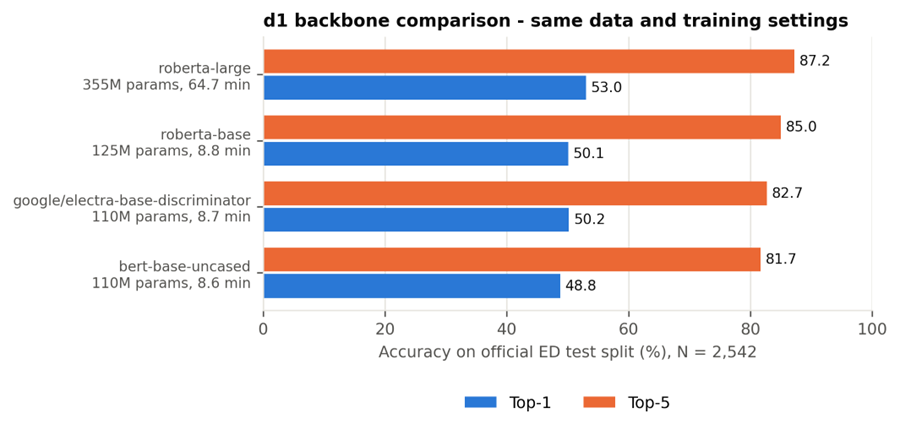
\includegraphics[width=0.95\linewidth]{figures/ch5_fig5.png}
\caption{Top-1 and top-5 accuracy of the detector candidates under identical training}
\label{fig:5.5}
\end{figure}

\subsection{Generator Alternatives}
\label{sec:5.2.3}

The generator determines how well the rules are adhered to, with Phi-4-mini at 65.3\% adherence, Qwen2.5-1.5B at 57.7\% and Gemma-3-4B at 22.0\%.

One might think that the most empathetic model of all is the instructive case, as it scores higher than Phi-4-mini on the empathy classifier and recognizes that 96.7\% of the time there is a feeling to recognize. However, it has an average of 133 words, 72\% of the responses exceed the limit and, in all the classifiers we measured, the system encourages longer responses (Section 5.4.4). Comparing similar length replies evens the playing field: in any band where both reply, Phi-4-mini holds up or just equals Gemma; and Gemma only outdoes Phi-4-mini at >120 words, where Phi-4-mini doesn't reply at all. Its apparent empathy is verbosity, and a system which is supposed to answer someone in distress, cannot disregard the length rule.

\subsection{Integration Alternatives}
\label{sec:5.2.4}

Making a connection between the two models is also a design decision - there are four different ways to do this and the difference lies in how much of the reasoning is asked of the generator. The two-stage design is able to enhance the emotion fidelity from 28.3\% to 36.7\% and the empathy from 4.89 to 5.05, which are reliable after correction, and shorten the replies from 80.4 words to 57.1 words, with the same detector and generator, and only the top-1 emotion and a general prompt. It requires 5.3 points in adherence to the rules which is an unreliable difference.

The benefit is dependent on the ability of the generator. The same change also affects Qwen2.5-1.5B, which drops adherence to 36.7\% and acknowledgement to 47.0\%, mirroring the results of the candidate-pick variant for this model (54.0\%): a small model provided with more room to reason becomes less compliant with the output format. The rules will not be dropped if a more detailed prompt is used; this can only be done with the bigger teaching-centered generator.

One drawback should be made explicit: this comparison involves the removal of three elements simultaneously: the top-3 selection, the emotion-specific guidance and the attention cues. The contributions of each of them were not distinguished, and it is listed as future work (Section 5.6.6) to separate them.

\subsection{Retrieval Augmentation}
\label{sec:5.2.5}

\textbf{How retrieval is used:} All the training conversations were inserted as a pair of messages with all-MiniLM-L6-v2 \cite{reimers2019sbert}. The detector's emotion was used to filter the pool of conversations to only those that contained the emotion at generation time, and the two most similar conversations (measured by cosine similarity) were retrieved and the human responses pasted on the system prompt as worked examples, above the same three rules \cite{lewis2020rag}. The second attempt further restricted the set to responses with a single question and explicitly reminded the person that the response must include one question mark.

\textbf{It reduced adherence to rules in both versions:} 54.3\% and 43.7\% compared to without retrieval (63.7\%). The explanation is in the data: only 4.3\% of the real listener replies adhere to all 3 rules, and what is retrieved is therefore a style that is contrary to the instructions provided in the same prompt. The percentage of compliance with the one-question rule was 76.0\% for the first version, and 57.0\% for the second version (after filtering examples and repeating the rule, the acknowledgement percentage dropped from 70.3\% to 57.0\%).

\textbf{Nothing was retrieved:} This is reported on all the same measures as all other systems because a design that sacrificed rule adherence may still be worth keeping if it gained in other aspects. It did not: empathy 4.85 compared to 4.80 without retrieval and emotion fidelity 27.7\% compared to 26.0\% both of which are very much smaller than the uncertainty on those estimates (Section 5.4.2) and the spread of its empathy scores is the widest of any system. It is the one design in Table~\ref{tab:5.1} that the model judges never scored. The three cells of the first attempt are not blank, but instead indicate that they cannot be recovered because their outputs were overwritten before the measures were computed. In this activity, participants can see examples of how people react in real life situations that go against explicit behavioural rules -- not reinforce them.

\begin{table}[htbp]
\centering
\scriptsize
\caption{Retrieval augmentation on every measure, against the same pipeline without it}
\label{tab:5.3}
\begin{tabularx}{\textwidth}{@{}lXXXXXX@{}}
\toprule
\textbf{Variant} & \textbf{Ack (\%)} & \textbf{One question (\%)} & \textbf{All rules (\%)} & \textbf{Mean words} & \textbf{WASSA empathy} & \textbf{Emotion validation (\%)} \\
\midrule
Without retrieval & 70.3 & 87.3 & 63.7 & 35.2 & 4.80 (SD 1.33) & 26.0 \\
With retrieval, attempt 1: 1-2 retrieved examples & not recoverable & 76.0 & 54.3 & not recoverable & not recoverable & not recoverable \\
With retrieval, attempt 2: filtered examples + rule reminder & 57.0 & 78.0 & 43.7 & 34.0 & 4.85 (SD 1.46) & 27.7 \\
\bottomrule
\end{tabularx}
\end{table}

\subsection{Assessment against Criteria beyond Performance}
\label{sec:5.2.6}

It's not just about performance and the other options differentiate clearly in that regard. These two designs, the fine-tuned baseline and the retrieval pipeline, are also the two that have the highest cost of change. All the single-model designs of any size have their emotional decision within, there is nothing to look at and nowhere to put a safeguard. The emotion is exposed in the decoupled designs, and the one picked is the most: three candidates, the picked one, the words that prompted it, the detector, the guidance and the generator are all separately replaceable.

The performance measures contradict each other and it is the two tables in Section 5.1 that resolve the issue of choice between the two. On what the replies do (Table~\ref{tab:5.1}) the final system is mid-table: it follows all three rules less often than the largest single model did or it was prompted to do, and it expresses the person's real emotion more often than any other system. In terms of how empathetic they are judged to be as it is second of eight, bettered only by the single model with 7.6 billion parameters, which requires 1.9 times its parameters and 62\% more GPU memory, and first among those that fit the requirement N1 in Section 3.1.2.

That's what the selected design is saying in so many words: at that scale, there's nothing more emotionally faithful than it, there's no system of that size that's rated more empathetic, and it's the only design here whose emotional decision can be read, logged or intercepted. What it loses is adherence to rules, and Section 5.5.5 quantifies just how much.

\section{Final Design Adjustments}
\label{sec:5.3}

Testing of the early pipeline, consisting of a GPT-2 Medium detector and a Qwen2.5-1.5B generator, revealed some flaws. Below are each of the adjustments that were made in response to a measured result, and each was re-evaluated on the same 300 conversations prior to being retained. 

\subsection{Adjustments to the Detector, the Generator and the Prompt}
\label{sec:5.3.1}

When the first detector was measured on the input that it receives, there was a mismatch between training and use: it was trained on situation descriptions of the dataset and in that case, the name of the feeling is nearly explicitly stated; in the case of the pipeline, it was given the user's conversational message. The detector was retrained on the first messages and, after the comparison of the encoders in Section 5.2.2, GPT-2 Medium was substituted by RoBERTa-base. Now it's accuracy is describing what it really does, and its ranking is good enough to be the top-3 selection.

Of the comparisons in Section 5.2, three were retained after being re-measured on the same conversations. \textbf{Replaced the generator:} Phi-4-mini obeyed the rules more frequently than Qwen2.5-1.5B, thus d2 was set to 4-bit version of Phi-4-mini.\textbf{ The emotion decision was made in its own call: }the correct emotion is in the top 3 of the detector in 76.5\% of the conversations, the top label is wrong in about half of the conversations, and an earlier version that decided and replied in a single call had harmed the rule-following. \textbf{There are 32 different emotions and guidance for each is fairly general:} "the user is feeling X". But what about a response to loneliness versus a response to pride? These combined, and with detector and generator fixed, yielded an increase in emotion fidelity from 28.3\% to 36.7\% and an increase in empathy from 4.89 to 5.05, both reliable after correction, with a 5.3-point drop in rule adherence not being reliable; replies also went down from 80.4 to 57.1 words, again within the limit.

The original design used an attention mechanism which was never implemented. However, a verification check revealed that the default implementation of attention in the library does not return any attention weights and does not throw any error, so the feature would have been silently inactive and seemed to be working. The adjustment includes an option to return weights, to stop if weights are not available, to merge adjacent fragments back into full words and to pass only the top 40\% of tokens (up to three phrases) so that the cues do not simply repeat the message.

\subsection{From Single Replies to a Conversation}
\label{sec:5.3.2}

This evaluation is based on 1 message and 1 response. A question that could not be assumed but had to be measured is how much of the conversation should the detector read if turned to the agent specified in Section 4.2.7?

\textbf{The reason why the dataset cannot answer it: }The maximum number of turns in EmpatheticDialogues conversations is 4, and the median is 2 turns, and the gold emotion does not change in the conversation, there is no multi-turn emotion shift in the data to tune a window against. Instead, we wrote conversations that include the kinds of changes that a real support conversation would generate, most notably the "I'm fine, actually I'm not" pattern, where the last message in the conversation communicates the opposite of how the person is really feeling. This is not statistical evidence, it is illustrative evidence for a design choice -- \textbf{this is our own opinion as to what a listener will hear in the column.}

\textbf{Across 10 short conversations,} with a deliberate change, moving from one turn to four shifted the prediction to what a listener in five of these would hear; in three the prediction was not changed; in two the prediction was changed -- one neighbour of the intended emotion was replaced by another -- but in none of the turns did a correct single-message reading become incorrect. The easiest example is the one that initiated this test - "I am okay. Well, not properly" is read as content at 72\% confidence, and "Someone yelled at me today very badly" with the previous turn as angry.

\textbf{However, a window can be too large:} Table~\ref{tab:5.4} opens up the window on four long conversations (6-8 turns), and four turns is the largest window that does not affect the quality of any of them. When six turns two of the four move away from the listener's reading, one of them, the break-up conversation, is correct at four turns (lonely, 61\%), but guilty at 64\% when the anger of the previous turns comes back into the window. With increased confidence, the control remains anxious at all widths, and the damage is not caused by the length of the input, but by stale emotions competing with the current one. We don't omit the burnout conversation, neither setting recovers it.

\textbf{The fixed 4-turn} window was kept as it gave the same answer as a 4-turn window that only widened when the detector was not sure, using the median of the detector confidence of 0.632 as the threshold in all 10 scenarios. The generator did not need this test as it is a large context window instruction following model, not a short text classifier.

\begin{table}[htbp]
\centering
\scriptsize
\caption{The same test on four long conversations, where a window can become too wide}
\label{tab:5.4}
\begin{tabularx}{\textwidth}{@{}lXXXXXXXX@{}}
\toprule
\textbf{Conversation} & \textbf{Turns} & \textbf{A listener would hear} & \textbf{Last 1} & \textbf{Last 2} & \textbf{Last 3} & \textbf{Last 4} & \textbf{Last 6} & \textbf{Last 8} \\
\midrule
work stress -> burnout -> quiet despair & 8 & devastated / empty - NOT ordinary work stress & content (50\%) & lonely (62\%) & ashamed (41\%) & lonely (20\%) & ashamed (49\%) & ashamed (54\%) \\
breakup -> anger -> loneliness & 7 & lonely / sad & anxious (31\%) & lonely (26\%) & lonely (40\%) & lonely (61\%) & guilty (64\%) & - \\
illness scare ending in relief & 7 & grateful / relieved & content (78\%) & content (36\%) & faithful (32\%) & hopeful (33\%) & faithful (25\%) & - \\
Control: emotion stays constant throughout & 6 & anxious (should stay stable at every window) & anxious (25\%) & anxious (30\%) & anxious (66\%) & anxious (75\%) & anxious (81\%) & - \\
\bottomrule
\end{tabularx}
\end{table}

A web demonstration of the agent was prepared for Hugging Face Spaces, with disclaimers and crisis resources shown on the page.

\subsection{Adjustments That Were Rejected or Deferred}
\label{sec:5.3.3}

Not all candidates' changes passed the evaluation. Retrieval augmentation reduced rule adherence from 63.7\% to 43.7\% and was rejected (Section 5.2.5), while a larger detector did not improve any of the measures of reply quality within the pipeline, although it was 2.9 points more accurate when used alone (Section 5.4.3).

There were two changes that were \textbf{postponed.} The boilerplate rate of 58.7\% would likely be decreased with the introduction of a repetition penalty, but generating the boilerplate replies would have negated the judge scores and human-evaluation items already created on those. The first item of future work (in Section 3.4) is a pre-generation crisis filter, which must be installed before any public deployment.

\textbf{Fine-tuned baseline:} a monolithic LoRA baseline had a configuration mistake, which has been corrected. Averaging 200.7 words and 7.07 questions per reply, 99\% of its answers were padded with the end-of-turn token (which meant they were limited to 250), and the collator removed padding from the loss, so it wasn't trained to stop: We retrained it using the padding token from the model, added start-up check to abort training if the end-of-turn padding would be masked, and chose the best epoch based on the validation loss. The corrected model concludes its response normally, as its responses do not exceed the word limit (10.0 words, wherein none exceeded the word limit), and adheres to rules in 22.3\% of cases. All results given in this thesis refer to the corrected baseline; the original run itself is given here only as an error documented.

\section{Statistical Analysis}
\label{sec:5.4}

Some of the differences so far reported are large enough to build on, others are not. This section is a divider between the two.

\subsection{How the Tests Were Done}
\label{sec:5.4.1}

All 300 conversations are answered by every system, and every detector is tested on all 2,542 conversations, making all comparisons paired, and allowing for comparison conversation by conversation, not just in aggregate. In the case of binary (yes/no) responses, e.g., whether a reply followed all the rules or expressed the true emotion, we employ McNemar's exact test which examines only the conversations in which the two systems disagree. For scores (e.g., empathy scores, judge ratings) we apply the Wilcoxon signed rank test that makes no assumption about the shape of the distribution. For each comparison there is also a 95\% bootstrap confidence interval based on 10000 resamples with seed 42, so that the size of a difference is not only apparent, but also visible.

The final system is compared with seven baselines on each measure, so p-values are adjusted within each measure by the Holm-Bonferroni procedure. \textbf{A difference is considered real if the adjusted p value is < 0.05 and the confidence interval does not contain zero.} Independent group comparisons (e.g., error-propagation analysis) are made using Fisher's exact test and the Mann-Whitney U test instead.

\subsection{The Final System against Each Baseline}
\label{sec:5.4.2}

Figure~\ref{fig:5.6} displays all comparisons together: the difference between the final system and each baseline on the three headline measures and its confidence interval, coloured by whether it survives correction. It is woven with three patterns.

\textbf{Empathy and emotion fidelity is reliably enhanced on each and every similar design.} The empathy score is higher than all baselines (except the largest single model) by 0.16 to 0.25 points, and\textbf{ by 0.30 points over the same generator alone }(95\% CI [+0.19, +0.41], adjusted p < 0.001). Emotion fidelity is also increased compared to all baselines except the largest single model (8.3 to 18.3 points, all adjusted p < 0.013). The improvements are not due to the size of the generator as the single-model baseline based on our own generator performs no better than the 1.5 billion parameter generator on these two measures (Section 5.5.5).

\textbf{We do not claim the difference between the rule adherence and the same-size single model after correction }(raw p-value of 0.032, Holm corrected p-value of 0.095). The final system is reliably better than zero-shot prompting, the fine-tuned model and the retrieval pipeline, no different from the initial pipeline or top-1 Phi-4-mini prompting, and reliably worse than its own generator used alone (-13.7, p = 0.002) and the largest single model (-22.3). It outperforms the same-size single question model by 19.0 points (p < 0.001) on the one-question rule alone.

\textbf{The one that has been corrected the most and is truly better on rules and empathy} is Qwen2.5-7B, which leads on overall rule adherence (+22.3 points), acknowledgement (+16.7), the one-question rule (+6.3) and empathy (+0.71). We report as it is.

\begin{figure}[htbp]
\centering
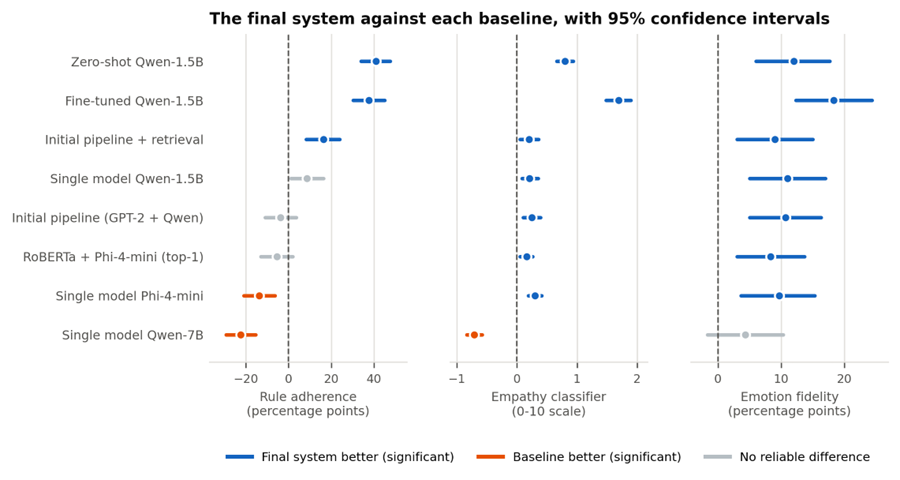
\includegraphics[width=0.95\linewidth]{figures/ch5_fig6.png}
\caption{The final system against each baseline on three measures, with 95\% confidence intervals}
\label{fig:5.6}
\end{figure}

\subsection{Is the Detector the Bottleneck?}
\label{sec:5.4.3}

The quality of the reply would be dependent on the accuracy of detection, and a better detector would result in better replies. Three tests declare it to be no.

\textbf{Replies based on a wrong label are no worse:} splitting each pipeline's replies by whether the detector matched the gold label shows no reliable loss of adherence of any pipeline: 61.2\% vs 66.0\% for the initial pipeline (p = 0.40) and no reliable difference for the final system (p = 0.096). Empathy is unaffected as well (4.83 against 4.78, p = 0.72).

\textbf{Replacing GPT-2 with the more accurate RoBERTa detector does not affect things downstream: }the emotion fidelity (p = 0.91) and adherence to rules (p = 0.09) do not change with the change of detector, but there is a significant difference between the two when they are used as classifiers.

\textbf{Similarly, doubling the detector did not make a difference:} When the detector was replaced with RoBERTa-large and the entire final system was rerun on the 300 conversations, the detector's accuracy improved by 3.0 points on the conversations, but nothing changed for adherence to the rules (p = 0.60), empathy (p = 0.85), emotion fidelity (p = 0.85), or the one-question rule (p = 0.60).

Here is one related result. The stage-1 choice is matched by the gold label in 42.3\% of the conversations, compared to the detector's 50.3\% (difference -8.0 points, CI [-13.3, -2.7] and p = 0.005), while the gold label is matched by the detector in 42.6\% (difference -7.7 points, CI [-12.9, -2.5] and p = 0.005). It is a real difference and the improvement of the two-stage design is not attributable to better emotion selection (Section 5.6.2).

All these together, detection accuracy is not what constrains reply quality, which is why it is worth spending the memory budget on the generator rather than the detector.

\subsection{What the Empathy Classifier Is Worth}
\label{sec:5.4.4}

The Spearman correlations range from 0.14 to 0.54, p < 0.02, with longer replies being more likely to be classified as empathy. Thus, a verbal system may appear empathetic, but not be, just as LLM judges have reported \cite{zheng2023judge}. This has an impact on two comparisons in opposite directions. It provides a complete explanation of the high score of Gemma-3-4B (Section 5.2.3). And it helps the final system's case over the top-1 prompting, because the final system gets the higher score with shorter replies (57.1 vs. 80.4 words). This also does not account for the largest single model, which has an average of 52.9 words for its replies.

Because of the dependence of a number of conclusions on the empathy classifier, we assessed its performance with the judges on the 512 replies scored. It correlates with the judges well (rho = 0.74) across systems, but it is in disagreement on one system: the single system developed on our generator is ranked 2nd by judge empathy and 7th by classifier score. Across individual responses, agreement is weak but genuine (rho=0.30, p<0.001) and does not disappear when length is controlled (partial rho=0.25), so it is not just a matter of a shared preference for long responses. The within-system agreement is weak (rho = 0.05 to 0.41, reliable in four of eight systems), compared to inter-judge agreement which is 0.69.

This is the proof on which we act throughout: the classifier compares averages of the system, never a single reply, and always against a second measure.

\subsection{What the Judges Separate, and How Much They Agree}
\label{sec:5.4.5}

Against the same-size single model the final system is rated reliably higher on empathy (+0.70, CI [+0.39, +1.01], p < 0.001), relevance (+0.44, p = 0.023) and overall (+0.44, p = 0.001), and reliably higher overall than the initial pipeline (+0.65), zero-shot prompting (+1.18) and the fine-tuned model (+2.73), all p < 0.001. Compared to the largest single model it is lower on empathy (-0.30) and overall (-0.21); however, neither of these differences is significant after correction (p = 0.073 and p = 0.109). \textbf{The judges do not differentiate between the three systems using the same generator at all: }top-1 prompting (overall +0.04, p = 0.71) and that generator alone (overall -0.10, p = 0.16).

The two judges' own correlation is rho = 0.69 for empathy and 0.68 overall, and their rankings of the eight systems are identical except for one pair that differ by 0.03. The literature suggests that they should be drawn from different model families to avoid bias from a single model \cite{verga2024}, which is what we have done.

\subsection{Human-Evaluation Statistics}
\label{sec:5.4.6}

All forty participants completed the study and none were excluded as they all consented. Each participant rated all three systems in all eight situations; thus, differences in rating systems cannot per se create an effect because a person who rates all three systems as such is doing so. The tests are therefore Wilcoxon signed-rank tests on per-participant mean ratings, with the Holm correction across the nine tests (three system pairs and three scales), and 10,000-sample bootstrap confidence intervals with the same seed as used elsewhere. Each of the six comparisons made with the final system is significant after correction, and none of the confidence intervals contain zero. Against the same-size single model it gains 0.64 points on empathy (95\% CI +0.41 to +0.88, adjusted p = 0.0001), 0.60 on contextual relevance (+0.33 to +0.88, adjusted p = 0.0017) and 0.65 on supportiveness (+0.41 to +0.89, adjusted p = 0.0002). Against the larger single model it gains 0.46 on empathy (+0.25 to +0.69, adjusted p = 0.0015), 0.47 on relevance (+0.25 to +0.71, adjusted p = 0.0039) and 0.50 on supportiveness (+0.29 to +0.72, adjusted p = 0.0008). After correction, the two single models cannot be distinguished from each other on any scale, and the additional parameters of the larger model do not provide any measurable improvement in the people's rating of its replies.

The final system was selected 196 times out of 320 on the preference question, 61.3\% (95\% interval 55.7\% to 66.6\%) which a 2 sided binomial test shows is far from the chance rate of a third (p<0.001). The larger single model was selected 21.6\% of the time and the same size model 17.2\% of the time, both also significantly different from chance, but in the opposite direction. The result is not dependent on a few situations or a few persons: the final system was preferred in all eight situations by 18 to 29 of the 40 persons and 22 of the 40 persons gave it their own highest average rating, as compared to 9 persons each of the two baselines. There is little consensus among participants and this is not set aside. Intraclass correlation for the 1-5 ratings is 0.084 for empathy; 0.075 for relevance; and 0.082 for supportiveness; and Fleiss' kappa for the preference question is 0.018. When correctly interpreted, these say that the rating that any one person gives to any one person contains little information, but that the preference is a consistent mild majority in every situation, and not a strong consensus in any situation; there is no situation in which most of the raters agree on the same reply for the same reason. What the study demonstrates is the sum total, and the sum total is in the same direction for all eight situations, on all three scales and the paired tests. Human ratings and the model judges agree where they overlap. The two are also correlated at a Spearman's rho of 0.516 (p = 0.049) and a Pearson's r of 0.537 (p = 0.039) over the 15 system-situation pairs that the judges also rated, and both rank the three systems in the same order: the final system first, the larger single model second, and the same-size model third. The judges give the end result of the final system 8.7 and the bigger single model 8.6 in those five cases. This is why the overall preference of the panel for the larger model, as reported in Section 5.1.5, is obtained. The wider judged set and not from the situations people saw.

\subsection{Limits of the Analysis}
\label{sec:5.4.7}

All of the above are subject to three limits. The 300-conversation sample will have a greater ability to detect a few percentage-point differences but less ability to detect smaller differences, and the 64-conversation judge sample has even less ability to detect differences. Emotion fidelity is based on our own detector reading text it has never seen. Within each measure, and only within each measure, Holm correction was applied, and the seven baselines were treated as one family of comparisons; that is a choice, and we state it rather than leave it implicit.

\section{Comparisons and Relationships}
\label{sec:5.5}

In this section, the results are compared with published work, where it is appropriate, and the relationships between variables uncovered by the experiments are reported.

\subsection{Compared with Published Work}
\label{sec:5.5.1}

The results of our detector are compared with the published results in Table~\ref{tab:5.5} on the same 32 emotions. When reading it, two things must be kept in mind: what the system reads, which may be a whole conversation, the situation description or only the speaker's first message; and which partition the number is from.

Our detector's 50.3\% exceeds every joint recognition: and-generation model listed, at 30.6-41.2\% \cite{lin2019moel,majumder2020mime,sabour2022cem,zhou2023case}, and the personality-aware models at 45.4-48.3\% \cite{wu2025traits}. There are four reasons for that and only the last is a choice we can take pride in.

\textbf{1. Our detector is initialised from a much stronger encoder:} pre-trained on approximately 160 GB of text, whereas MoEL, MIME, CEM and CASE initialise their word representations from GloVe vectors and train their encoders only on EmpatheticDialogues. The only joint model in the table, which is built on pre-trained components, is RoBERTa-GPT2, which is the only one that matches us.

\textbf{2. It does one thing:} Our joint model is trained and selected on emotion recognition as an auxiliary task and shares its capacity with response generation, while the joint models learn emotion recognition as an auxiliary task only.

\textbf{3. It is selected based on the measure it is being used for: }The checkpoint saved is the one with the best validation accuracy and the candidate selected is the one with the best top-5 accuracy, since the design uses a ranking, not a single label.

\textbf{4. It is trained on the text it will actually be given: }Training on the situation description, as the first version of this project did, reads as a better number and is a worse detector: the same model loses about nine points when moved to the message a user really writes (Section 5.3.1).

The fair summary is that it achieves this accuracy when it reads less, one message, not a full conversation, as would a live system.

\begin{table}[htbp]
\centering
\scriptsize
\caption{Emotion recognition on EmpatheticDialogues in published work and in this thesis}
\label{tab:5.5}
\begin{tabularx}{\textwidth}{@{}lXXXX@{}}
\toprule
\textbf{System} & \textbf{Input and split} & \textbf{Top-1 (\%)} & \textbf{Top-5 (\%)} & \textbf{Source} \\
\midrule
EmpDG (Li et al., 2020) & Joint model, full conversation & 30.64 &  & Qian et al. 2023, Table 1 \\
MoEL (Lin et al., 2019) & Joint model, full conversation & 30.75 &  & Qian et al. 2023, Table 1 \\
MIME (Majumder et al., 2020) & Joint model, full conversation & 31.21 &  & Qian et al. 2023, Table 1 \\
KEMP (Li et al., 2022) & Joint model, full conversation & 36.57 &  & Qian et al. 2023, Table 1 \\
CEM (Sabour et al., 2022) & Joint model, full conversation & 37.81 &  & Qian et al. 2023, Table 1 \\
CASE (Zhou et al., 2023) & Joint model, full conversation & 38.92 &  & Qian et al. 2023, Table 1 \\
ESCM (Yang et al., 2023) & Joint model, full conversation & 41.19 &  & Findings of EMNLP 2023 \\
Personality-aware model (Wu et al., 2025) & Joint model, text-only ED & 45.4 &  & COLING 2025 main.598, Table 4 \\
EmpSOA & Joint model, text-only ED & 48.3 &  & COLING 2025 main.598, Table 4 \\
fastText (Rashkin et al., 2019) & Classifier, situation description & 43.0 &  & ED paper \\
DeepMoji (Rashkin et al., 2019) & Classifier, situation description & 48.0 &  & ED paper \\
OURS - RoBERTa-base d1 & Classifier, first utterance, TEST split & 50.3 & 84.3 & this work \\
\bottomrule
\end{tabularx}
\end{table}

By contrast, published generation scores cannot be compared with ours: their test set is much bigger, and the scores drop as the test set increases, from 32.3\% at 50 replies in their test set to 15.6\% at 300; whereas published BERTScore values refer to a reply that is compared with a reference answer that comes after a multi-turn context. Thus, we report measures that are not found in published work, such as rule adherence, an independent empathy classifier, emotion fidelity and paired significance tests.

Human evaluation enables comparison of direction, if not of size: people in published studies strongly prefer LLM replies to those of purpose-built empathetic models, rating ChatGPT at 4.64 out of 5 compared to 3.08 for CEM \cite{qian2023llm}.Our own study confirms this and takes one step further: the 40 participants preferred the final system in 61.3\% of the choices, a single model almost twice the size in 21.6\% of the choices, and a single model of its own class in 17.2\% of the choices, and rated it higher on all three scales. We have seen that a small general model with a separate emotion detector is preferred to a larger general model without an emotion detector, whereas published work shows that a large general model is preferred to a small purpose-built model. The protocols vary, so 5-point ratings, A/B preferences and our 3-way choice are only comparable in terms of direction.

\subsection{What Detector Accuracy and Generator Capacity Each Buy}
\label{sec:5.5.2}

In all three tests of Section 5.4.3, the user never received a gain of more than 2 to 3 points in the detection accuracy. The key is in the shape of the errors: an answer for\textit{ terrified} when the person was \textit{afraid }is still an answer for fear, and the same nearness is what makes the top-3 candidate set worth passing on, as opposed to the single most probable, which was correct only 50.3\% of the time. The emotion fidelity increase was more important than the accuracy of the finding: per-emotion two-stage prompting increased the emotion fidelity by 8.3 points, which is more than any detector upgrade we tested, with detector and generator unchanged.

Only a generator capable of following the richer prompts will be helped by the richer prompts. The same additions that leave Phi-4-mini's rule adherence unchanged while raising its empathy and emotion fidelity lower Qwen2.5-1.5B's adherence from 57.7\% to 36.7\% (Section 5.2.4), the earlier candidate-pick variant showed the same pattern on the smaller model, and adherence under a plain single-model prompt climbs from 51.3\% at 1.5 billion parameters to 82.3\% at 7.6 billion. The implication is that the complexity of instruction should be aligned with the capacity of the generator, and that in the case of less than a few billion parameters, it is better to choose a simpler prompt.

\subsection{Cost: Parameters, Memory and Time}
\label{sec:5.5.3}

Parameters by themselves don't determine the cost of running a system, as the system loads two models and calls the generator twice in every reply. Hence, we have measured the peak GPU memory and response time for the final system and both single models on the same 50 conversations, on the RTX 4060 used throughout. The measurements are provided in Tables 5.30-5.33, and are compared to the other systems in Table~\ref{tab:5.6}.

The final system achieves \textbf{97.5\%} \textbf{of the overall judge score} at 52.0\% of the parameters of the Qwen2.5-7B single model, maintains 87.7\% of the empathy-classifier score and 72.9\% of the rule adherence, and surpasses it on emotion fidelity. It does this with \textbf{38\% less peak GPU memory,} and no statistically significant difference in response time (CI [-0.03, +0.56] s, p = 0.10); per generated token the two are virtually indistinguishable (65.7 ms vs. 65.4 ms; p = 0.91). The additional operations of the decoupled design are inexpensive: detection + cue extraction = 0.016 s, and the stage-1 call = 0.29 s, or approximately 7\% of the time per reply.

These are two honest qualifications. The Qwen2.5-1.5B single model is lighter (2.90 GB) and 2.6 times faster, so the final system is efficient relative to the large model whose quality it approaches, not relative to the smallest baseline, whose replies are reliably less empathetic. The measurements are for one GPU and 50 messages and therefore indicative only.

\subsection{Do the Response Rules Measure Something That Matters?}
\label{sec:5.5.4}

One of our headline measures is adherence to rules, and the rules themselves must be justified: It's only a virtue to adhere to the rules if the rules are for something worth doing. The origin of each rule, and the measured effect, which is calculated within each system by subtracting the mean of that system and the effects cannot be due to differences between systems.

\textbf{Acknowledging the feeling} is the \textit{emotional reactions} mechanism of EPITOME is a framework of empathy in text-based support that is based on existing empathy scales \cite{sharma2020epitome} and the mechanism of emotional reactions is the acknowledgement of the feeling. Within the same system, in our data, replies that acknowledge score 0.36 points higher on the empathy classifier (p < 0.001, 3,300 replies); the judges point the same way but not reliably.

\textbf{A single question is a balance between two things: }a reply with no question, and several questions, which counselling guidance warns against \cite{samhsa2019tip35} and which only 4.7\% of the listener replies in the dataset do. \textbf{There is no automatic reward for this rule,} so we offer it as a usability and safety requirement, which can be seen in the failure mode of the fine-tuned baseline, and not as a way to a higher score.

\textbf{Keep a reply to within 120 words} so it is easy for someone in distress to read. The two measures disagree here: the judges rate the replies in the same system 0.65 points higher on empathy (p = 0.006), while the classifier rates them 0.22 points lower, the known length preference of the classifier. We follow the judges, since they read the text, not a proxy that is sensitive to length.

To summarise, two of the three rules are supported by published practice and our own data, and the third is supported by practice but not our automatic measures. The only test to settle it is the human study, which is ongoing.

\subsection{What the Detector Itself Contributes}
\label{sec:5.5.5}

All comparisons so far have been with a fixed generator, but with varying conversations and decoding. The test that isolates the design provides the final system's own generator with the single-model prompt and no detector whatsoever. The result is illustrated measure by measure in Figure~\ref{fig:5.7}, as the single model writes 29\% longer replies.

\textbf{The gains belong to the design, not to the generator: }Switching from Qwen2.5-1.5B to Phi-4-mini as a single model increases rule adherence significantly (51.3\% to 73.7\%, p < 0.001), but does not increase empathy (4.84 to 4.75, p = 0.18) or emotional fidelity (25.7\% to 27.0\%, p = 0.70), so a larger generator alone does not purchase the empathy we report. The three candidates and the per-emotion guidance, when added to the same generator, result in an increase of empathy to 5.05 (p < 0.001) and emotion fidelity to 36.7\% (p = 0.007). The empathy gain is the more robust of the two: it persists with shorter replies and increases with length control; the fidelity gain, by contrast, decreases with length control (p = 0.13).

\textbf{The price is adherence to the rules,} the decoupled system adheres to all three rules less frequently (60.0\% vs. 73.7\%, p = 0.002), mostly by acknowledging it, and the one-question rule is not different, while every reply is within the length limit, with the generator fixed. The reason is that the rules are included in the prompt, and the per-emotion guidance and cue words are included in the prompt, too, but the single-model prompt includes only the rules. When length is kept constant, the acknowledgement difference is gone (p = 0.36) and the rule difference is just on the edge of significance (p = 0.04), meaning that part of the cost is length and part is real. The judges' scores are virtually indistinguishable (8.68 versus 8.78, p = 0.16), and are virtually the same at matched length.

The trade-off is that at an equal generator, the decoupled design will be more expressive of the person's emotion, will be more successful on an independent empathy classifier, will repeat itself less and write shorter replies, and will allow for logging, auditing or intercepting of the emotional decision, while paying for that with some adherence to the rules. It's an exchange, not a clean win and we're reporting it as such.

\begin{figure}[htbp]
\centering
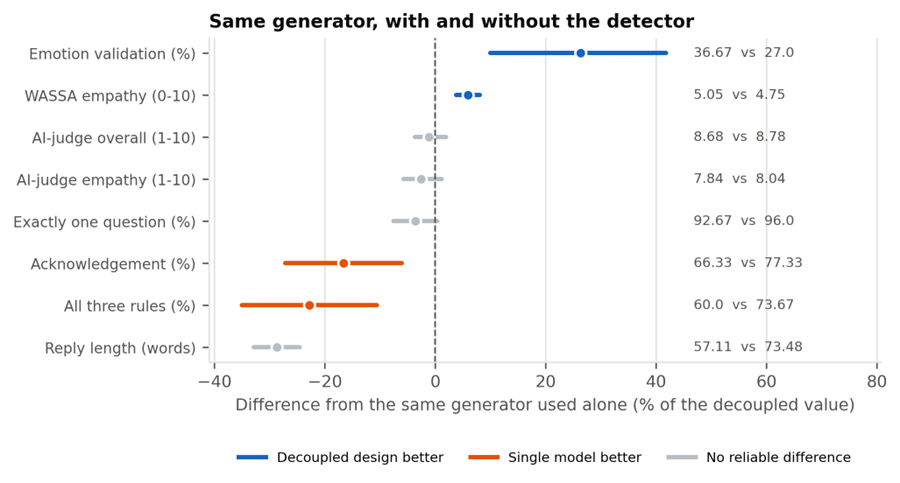
\includegraphics[width=0.95\linewidth]{figures/ch5_fig7.png}
\caption{The decoupled design against the same generator used alone, measure by measure}
\label{fig:5.7}
\end{figure}

\section{Discussion}
\label{sec:5.6}

This section reads the results as a whole -- what they said about the research question, why the surprising results came out that way, what the research cannot claim and what should come next.

\subsection{Answer to the Research Question}
\label{sec:5.6.1}

The question of the thesis was whether emotion detection and response generation can be separated to get better empathetic responses than a single model for both being asked on a single consumer GPU. The answer is a qualified yes, and the entire answer is in Table~\ref{tab:5.6}: our system, the same generator alone (which disconnects the design), and the larger single generator (the strongest that fits the hardware).

There are three true and one false statements in that table, read down the table. \textbf{It is parameter efficient}, being 52\% of the size of the larger model, and ranking second on the empathy panel of eight systems. \textbf{It is resource-efficient:} It's efficient with its 3.40 GB of GPU memory compared to 5.47 GB, and there's no consistent difference in its response time. \textbf{It is more emotionally faithful than either:} 36.7\% of its replies express the person's true feeling compared to 32.3\% and 27.0\%, and it repeats itself less than the same generator alone, while writing 22\% fewer words. What it doesn't score well at is rule adherence: 60.0\% to 73.7\% and 82.3\% and we don't say otherwise. Two cells are blank because we did not measure the single Phi-4-mini baseline, and do not attempt to estimate it.

\begin{table}[htbp]
\centering
\footnotesize
\caption{The three systems a reader has to choose between, measure by measure}
\label{tab:5.6}
\begin{tabularx}{\textwidth}{@{}lXXX@{}}
\toprule
\textbf{What a reader wants to know} & \textbf{Our system} & \textbf{The same generator alone} & \textbf{The bigger single model} \\
\midrule
What is it? & A detector and a generator, two short calls per reply & One model, one call per reply & One model, one call per reply \\
Models it loads & RoBERTa-base + Phi-4-mini (4-bit) & Phi-4-mini (4-bit) & Qwen2.5-7B (4-bit) \\
Total parameters & 3.96 billion & 3.84 billion & 7.62 billion \\
Peak GPU memory & 3.40 GB & not measured & 5.47 GB \\
Seconds per reply & 4.17 s & not measured & 3.91 s \\
Follows all three rules & 60.0\% & 73.7\% & 82.3\% \\
Empathy classifier (0-10) & 5.05 & 4.75 & 5.76 \\
Reply expresses the true feeling & 36.7\% & 27.0\% & 32.3\% \\
Empathy panel (three raters, combined) & +0.59 (2 of 8) & +0.53 (3 of 8) & +1.11 (1 of 8) \\
Replies using a stock phrase & 58.7\% & 72.3\% & 58.7\% \\
Words per reply & 57 & 73 & 53 \\
Shows which emotion it answered & Yes: three candidates, the chosen one, and the cue words & No & No \\
A safeguard can run before the reply is written & Yes & No & No \\
\bottomrule
\end{tabularx}
\end{table}

The empathy and fidelity gains are not due to the size of the generator, but to the structure, which is what the middle column represents: the same generator alone scores 4.75 and 27.0\%, and it does not gain anything on either measure when compared to the single model with 1.5 billion parameters (Section 5.5.5). The larger single model still outperforms on rules and on the empathy classifier, but the judges don't distinguish its empathy or its overall score from ours post-correction. So the argument for decoupling is not that separation is better than scale. It is about that separation, writing down an emotional decision that fits the hardware most people have.

\subsection{Why the Two-Stage Design Works}
\label{sec:5.6.2}

The most surprising result in the chapter is that the stage-1 choice is even less like the label in the dataset than the detector's own top choice (42.3\% vs 50.3\%), yet the system based on the stage-1 choice has the highest emotion fidelity and the highest empathy scores of any comparable system. This is reconciled by three observations.

First, EmpatheticDialogues assigns each conversation exactly one fine-grained label, which the speaker selects prior to writing anything; many messages seem to express a neighbouring feeling; since almost all disagreements are between neighbours, a choice that differs from the selected one label is often still a fair reading of the text. Second, replies based on a mislabeled label are as good as replies based on a correct one (Section 5.4.3): it is not the gold label per se that a reply requires, but the feeling of closeness to answer. Third, the improvement is apparent when per-emotion guidance is added. When you tell the generator how to answer loneliness, you change the answer from lonely to something else.

Since the selection and the guidance and cue words together were removed in our comparison, the percentages of the individual components are not distinguishable, but the accuracy result above indicates that the guidance is the most important component. This is also a smaller effect than the design's edge over single models, as there is little difference in the judges' assessment of the two-stage and top-1 variants, and the edge is seen in the finer measures of empathy and emotional fidelity.

\subsection{Objections, and When a Single Model Is the Better Choice}
\label{sec:5.6.3}

There are two objections which may be raised in this design and which were tested but not argued. 

\textbf{That a second model was not needed: }a model of the same size, and our own generator trained similarly, was equally unempathetic and unwarm in its responses; the detector was 125 million parameters, and a larger model would not affect the conclusion. Because real listener responses rarely adhere to the rules. 

\textbf{Retrieval would do the job more simply:} to manifest the generator the same emotion \cite{lewis2020rag} cut rule adherence in both the versions we built. We haven't developed the entire agentic system that was proposed to us, this evidence is about retrieval-augmented prompting, not agentic designs in general.

There's a case against our design, too. Given the sole objective of the best reply, our results on hardware which can store a 7-billion-parameter model are in favor of the larger single model. Decoupling should be used when the emotional reasoning must be evident: To audit the reason why a reply was written in a given way, to indicate to a user or a clinician what emotion was read, before any text is generated, or when components need to be replaceable individually. The two are not mutually exclusive, but the next most obvious experiment is to combine the detector and per-emotion prompting with a larger generator.

\subsection{Limitations}
\label{sec:5.6.5}

This work is constrained by seven limitations.

\textbf{Data:} EmpatheticDialogues is English, crowd-sourced and single-labelled, meaning that detection accuracy and suitability of the replies may not be held to transfer to the Bangla speakers and to those in real distress.

\textbf{Safety:} Suicidal ideation is not a label set, and there is no crisis safeguard other than interface disclaimers.

\textbf{Measures:} All automatic measures are proxies, the acknowledgement check is keyword based, the one-question rule is not rewarded by either empathy measure, the classifier has been trained on another domain and the length dimension, the judge panel currently consists of 2 members and the emotion fidelity is based on our own emotion detector.

\textbf{Number of conversations for generation:} 300; for judges: 64; and human study: 40 participants over 8 situations..

\textbf{Single turns:} The quantitative results are all basically for single turns, and the multi-turn agent was only evaluated on scenarios.

\textbf{Repetition:} 58.7\% of responses are repetitions of stock phrases.

\textbf{Efficiency:} Memory and time were measured for one GPU for 50 messages.

\subsection{Future Work}
\label{sec:5.6.6}

\textbf{Immediate Priorities}

\textbf{Incorporate a pre-generation crisis filter:} The filter is a ``must'' before public deployment and has reviewed safe responses \cite{who2023suicide}.

\textbf{Perform a component-wise ablation:} Perform an Ablation Study which unconfounds emotion selection, per-emotion guidance, and attention cues.

\textbf{Use a larger model generator:} Use the detector and per-emotion prompting with a larger generator model.

\textbf{Guidance written with practitioners:} three universal rules from published sources (Sharma et al; SAMHSA), and per-emotion guidance was not from published sources.The one part without any clinician is written by the authors external grounding. It needs to be created with practising Counsellors and Clinical. By interviewing them about their reactions to each type of situation, psychologists are able to assess a person's response style.requesting them to rewrite the 32 sets of instructions, and noting when their practice disagrees with ours, such an interview is not about any patient's, it is about professional practice, records. Already, these systems have been evaluated in published works based on counselling criteria.against clinicians themselves [Loh \& Raamkumar; Sorin et al.], and the standard is presentour guidance has not been kept to. The change is cost-effective as the guidance is Generation-time read is not followed by rewrite, which is no-training.

\textbf{Beyond English (Language Extension)}

\textbf{Compile localized data:} Obtain or create emotion-sensitive Bangla labelled conversations, including the naturally occurring code-mixed Bangla-English that people type.

\textbf{Retrain the detector:} trained from multilingual encoder with 125M Parameters, which is still still very low cost from a computational perspective.

\textbf{Rewrite per-emotion guidance:}Develop own guidance with native speakers, not translating guidance from English, and ensuring cultural correctness about the way in which emotions are addressed (e.g., loneliness, shame). (The separated architecture will enable it to retain the same generator while just changing the detector and guidance).

\textbf{Subsequent Steps}

\textbf{Control repetition:} Control text repetition in particular during the decoding time.

\textbf{Evaluate on real data:} Evaluate the system for actual multi-turn conversations and collect assessments from mental health professionals.

\textbf{Measure hardware performance:} Benchmark memory usage and response times for alternative hardware, such as CPU-only and mobile devices.

\chapter{Conclusion and Future Work}
\label{ch:6}

\section{Summary of Findings}
\label{sec:6.1}

The goal of this research was to create an empathetic response system that is separated between emotion detection and response generation, to fit the entire system within the 8 GB of an ordinary consumer graphics card, and to measure whether or not the separation is worthwhile. From the 4,200 scored replies in fourteen configurations, the answer is a qualified yes, and the qualification is as straightforward as the support. The work is split in two parts. The first constructed the detector. Five encoders and decoders were trained in the same way, and the results of RoBERTa-base were chosen: 50.3\% top-1 accuracy and 84.3\% in the top-5 for the 32 emotions of EmpatheticDialogues, outperforming all jointly trained models published on this corpus. There are two findings that are more important than that number. Near neighbours are almost always the only mistakes the detector can make, for example, afraid is read as terrified, and sad is read as devastated; and in fact, what it is trained on is more important than which network is selected, as training on the situation descriptions of the corpus while using it on the user's own message cost around nine points. Both lead to passing three candidate emotions instead of one.

The second part constructed and tested the pipeline. Five different methods of connecting the two models were measured and compared to the detector, with the prompt fixed, and three generators were compared with the detector and prompt held fixed. The chosen design, which sees Phi-4-mini first select one of the three detector candidates and then write under per-emotion guidance, comes in second place of the eight systems with an empathy score of +0.59 versus +1.11 for a single model that is nearly double the size. The argument is carried in two comparisons. The same generator alone scores +0.53, so the gain is due to the design rather than the size of the generator; and the system scores 11.0 points higher than a single model of similar size, and 36.7\% of the replies are the speaker's true emotion. It does this using 3.40 GB of peak memory, 3.96 billion parameters and 4.17 seconds per reply, which is 38\% less memory than a single model, with 1.9 times the parameters and at no significant cost in response time. The human study confirms the comparison of the automatic measures that was left open: 40 participants rated the two-stage system highest on all three scales and preferred it in 61.3\% of the choices, compared to a single model that is almost twice the size in 21.6\% of the choices.

There are four findings that qualify the claim. The biggest single model is still leading on the empathy panel, and if it's deployed with the hardware to run a 7-billion-parameter model, and no need for an auditable emotional decision, it should use one. The system has its own three response rules, which takes up 60.0\% of the prompt space, versus 73.7\% for the same generator alone, as the rules share prompt space with the emotional guidance. Whether or not the two model judges distinguish the two configurations, the case is decided based on the empathy classifier, emotional fidelity, lower repetition and the visible decision, not on judge preference. But with the detector replaced by a more accurate one, three points better on the same test, no measure of reply quality changed, meaning that the detector was not the limiting component.

\section{Contributions to the Field}
\label{sec:6.2}

There are six contributions to this research. 
\textbf{First and foremost,} it gives you a calibrated understanding of what you're paying for and what you're paying for in a scale where it actually matters when you go for a "decoupled" design. The combination of a small emotion model and a large language model has been proposed earlier, but not tested against a hardware constraint of models of similar size and larger models, as this is the real-world choice one might face when deciding how to construct such a model.

\textbf{Second,} it makes note of negative outcomes, which can save other research workers time. A detector which was 3 points more accurate showed no improvement on any measure of the reply, suggesting the value of the detector is in the structure it provides, not in the precision of the label, and that further accuracy is not where the remaining gains lie. Similarly, retrieval augmentation (which was added on the reasonable expectation that related passages would help) led to a decrease in adherence to rules, from 63.7\% to 43.7\%, and did not help performance.

\textbf{Third,} it allows the emotional decision to be heard. Each response includes the three candidate emotions, the selected emotion and the phrases that triggered the emotion. An end-to-end model can provide a similar response, but it will not indicate its response -- and if a response is incorrect, there is no mechanism to secure a safeguard and no mechanism to review: in a sensitive domain, a difference of kind, not just degree.

\textbf{Fourth,} it provides an evaluation design that can be re-used in other work on this task. It does not rely on similarity to a single reference reply, but rather integrates three elements: explicit evaluation of the parts that a supportive reply must include; an empathy panel that compares two model judges from different developers and compares a classifier trained directly from human ratings; and paired statistical Testing with correction for multiple comparisons, which renders a difference as real only if it is detected by both the modified test and the confidence interval.

\textbf{Fifth}, it does not provide a benchmark entry; the context window for the detector, the memory for the generator and rules are relaxed after the first turn, preventing an interrogation of the conversation.

\textbf{Sixth,} it records the practical failures that a reproduction will reproduce, such as a fine-tuning defect: a reproduction of the model will not learn to stop if the wrong padding token is used, along with an attention implementation that does not return any weights at all.

\section{Limitations}
\label{sec:6.3}

There were seven limitations that restricted these conclusions as described in detail in Section 5.6.5. This is an English-language, crowd-sourced corpus with one label per conversation, so nothing said here should be taken as representative of Bangla language speakers or persons in actual distress. Label set doesn't include a category for suicidal ideation and there's no crisis safeguard in the system. All automatic measures are proxies: the acknowledgement check is looking for keywords, the empathy classifier is trained in a different domain and favours longer answers, emotional fidelity is being assessed by our own detector. The evidence is based on 300 conversations, 64 of which were viewed by the judges, and a small study of 40 people, whose ratings matched. All quantitative results are related to first replies as the multi-turn agent was not measured, but checked on scenarios. The figure for repetition is still high with 58.7\% of replies. The cost figures are from one graphic card, more than 50 messages.

\section{Recommendations for Future Work}
\label{sec:6.4}

\textbf{Immediate extensions:} A crisis filter that checks the message prior to generation and provides answers from a set of reviewed safe responses is necessary before this system is placed in front of anyone and is the first piece of work we recommend \cite{who2023suicide}. Next, a component-wise ablation where the three things the pipeline provides at once (emotion choice, per emotion guidance and the attention cues) are separated, and the contribution of each is known instead of inferred. The rule-adherence gap shall be bridged by checking and repairing the reply after it's written, and repetition shall be controlled at the decoding time, both of which were intentionally deferred here to keep the evaluated outputs fixed.

\textbf{Beyond English:} The decoupled structure is an advantage here, since a new language requires a new detector and a new guidance but not a new generator and the detector is only 125 million parameters. Three steps follow: collecting or adapting the emotional conversations in Bangla, including the code-mixed Bangla-English that people here actually type; retraining the detector from a multilingual encoder; and rewriting the per-emotion guidance with speakers of the language, as the nature of the question and answers would differ based on location and a translated prompt would bring English assumptions into the response. The literature of emotion classification with low resources indicates that the focus of the difficulty will be on the detector \cite{ed_github}.

\textbf{Stronger evaluation:} The evaluations should be made not only on individual responses but also on entire conversations evaluated by human evaluators and the human evaluation should be repeated at a size that allows statistical testing, ideally with mental-health professionals as evaluators. More members in the empathy panel would be nice, and the numbers of cost should be repeated on other hardware, such as machines without a graphics card, since it's about deployment.

\textbf{Final remarks:} This work is not about a new record on a benchmark and it wasn't designed to get one. It's in demonstrating, through measurement, not argument, that a system built from a small specialised model and a modest general one can be more emotionally responsive than a single model of the same size, can run on hardware already owned by the student so that a person's disclosure never leaves their machine, and can show exactly what it understood before it answers. How to arrange them will be more important than how big to make them, and a design whose emotional reasoning can be inspected and corrected and replaced one part at a time will be what a sensitive application will require, as capable open models continue to get smaller.


% ---------------------------------------------------------------------------
%  Bibliography.  Do not add a thebibliography block as well: a document may
%  have one or the other, never both.
% ---------------------------------------------------------------------------
\bibliographystyle{IEEEtran}
\bibliography{references}

\end{document}
